\documentclass{article}
\usepackage{amsmath,amssymb,graphicx,enumitem,wrapfig}

\begin{document}
\parindent=0cm
\parskip=6pt
\pagestyle{empty}

%Begin
%Language English
%Source Cariboo College High School Mathematics competition
%Title Junior Preliminary Round 1974
%Question 1
%Subject arithmetic
%Category integers
%Type MC
%Choices 5
%Answer D
%Creator Victor Semenoff
%Rdifficulty 18
%Qtext

\scriptsize
Source: Cariboo College High School Mathematics Contest

\normalsize
%\begin{wrapfigure}[2]{r}[0pt]{0pt}
%	\includegraphics[width=30mm,viewport=]{CCJ78-04}
%\end{wrapfigure}
If 18 divided into the number $n$ goes 30 times with remainder 2, then $n$ equals:\\
%ChoiceA
(A) 78\\
%ChoiceB
(B) 538\\
%ChoiceC
(C) 540\\
%ChoiceD
(D) 542\\
%ChoiceE
(E) 5402\\
%Ftext

%\begin{wrapfigure}{r}[0pt]{0pt}
%	\includegraphics[width=30mm,viewport=]{CCJ78-04}
%\end{wrapfigure}

\textbf{The correct answer is (D): 542}\\[1 ex]
From the question we have
\begin{align*}
\frac{n}{18}&=30+\frac{2}{18}\\
n&=18\times30+2=542.
\end{align*}
%End
\\[5 ex]
%Begin
%Language English
%Source Cariboo College High School Mathematics competition
%Title Junior Preliminary Round 1974
%Question 2
%Subject arithmetic
%Category integers
%Type MC
%Choices 5
%Answer A
%Creator Victor Semenoff
%Rdifficulty 19
%Qtext

\scriptsize
Source: Cariboo College High School Mathematics Contest

\normalsize
%\begin{wrapfigure}[2]{r}[0pt]{0pt}
%	\includegraphics[width=30mm]{CCJ78-04}
%\end{wrapfigure}
If 684,342 is divided by 9 the remainder is:\\
%ChoiceA
(A) 0\\
%ChoiceB
(B) 2\\
%ChoiceC
(C) 4\\
%ChoiceD
(D) 6\\
%ChoiceE
(E) 8\\
%Ftext

%\begin{wrapfigure}{r}[0pt]{0pt}
%	\includegraphics[width=30mm]{CCJ78-04}
%\end{wrapfigure}

\textbf{The correct answer is (A): 0}\\
The remainder when a number is divided by 9 equals the remainder of the sum of the digits of that number divided by 9. The sum of the digits of 648,342 is 27. Since the remainder when 27 is divided by 9 is 0, the remainder when 648,342 is divided by 9 is also 0.
%End
\\[5 ex]
%Begin
%Language English
%Source Cariboo College High School Mathematics competition
%Title Junior Preliminary Round 1974
%Question 3
%Subject arithmetic
%Category fractions
%Type MC
%Choices 5
%Answer D
%Creator Victor Semenoff
%Rdifficulty 15
%Qtext

\scriptsize
Source: Cariboo College High School Mathematics Contest

\normalsize
%\begin{wrapfigure}[2]{r}[0pt]{0pt}
%	\includegraphics[width=30mm]{CCJ78-04}
%\end{wrapfigure}
$\frac{(75)^2+3(75)}{25}$ equals:\\
%ChoiceA
(A) 18\\
%ChoiceB
(B) 84\\
%ChoiceC
(C) 90\\
%ChoiceD
(D) 234\\
%ChoiceE
(E) 450\\
%Ftext

%\begin{wrapfigure}{r}[0pt]{0pt}
%	\includegraphics[width=30mm]{CCJ78-04}
%\end{wrapfigure}

\textbf{The correct answer is (D): 234}\\[1 ex]
\begin{equation*}
\frac{(75)^{2}+3(75)^{2}}{25}=3\times78=234.
\end{equation*}
%End
\\[5 ex]
%Begin
%Language English
%Source Cariboo College High School Mathematics competition
%Title Junior Preliminary Round 1974
%Question 4
%Subject geometry
%Category area
%Type MC
%Choices 5
%Answer E
%Creator Victor Semenoff
%Rdifficulty 17
%Qtext

\scriptsize
Source: Cariboo College High School Mathematics Contest

\normalsize
\begin{wrapfigure}[2]{r}[0pt]{0pt}
	\includegraphics[width=30mm, viewport=29 173 491 578]{CCJPR74-4pic.eps}
\end{wrapfigure}
The radius of each of the semicircles in the figure is 4, and AB=CD=4. The area of the figure is:\\
%ChoiceA
(A) $32+16\pi$\\
%ChoiceB
(B) $64+16\pi$\\
%ChoiceC
(C) $32+8\pi$\\
%ChoiceD
(D) 32\\
%ChoiceE
(E) 64\\
%Ftext

\begin{wrapfigure}{r}[0pt]{0pt}
	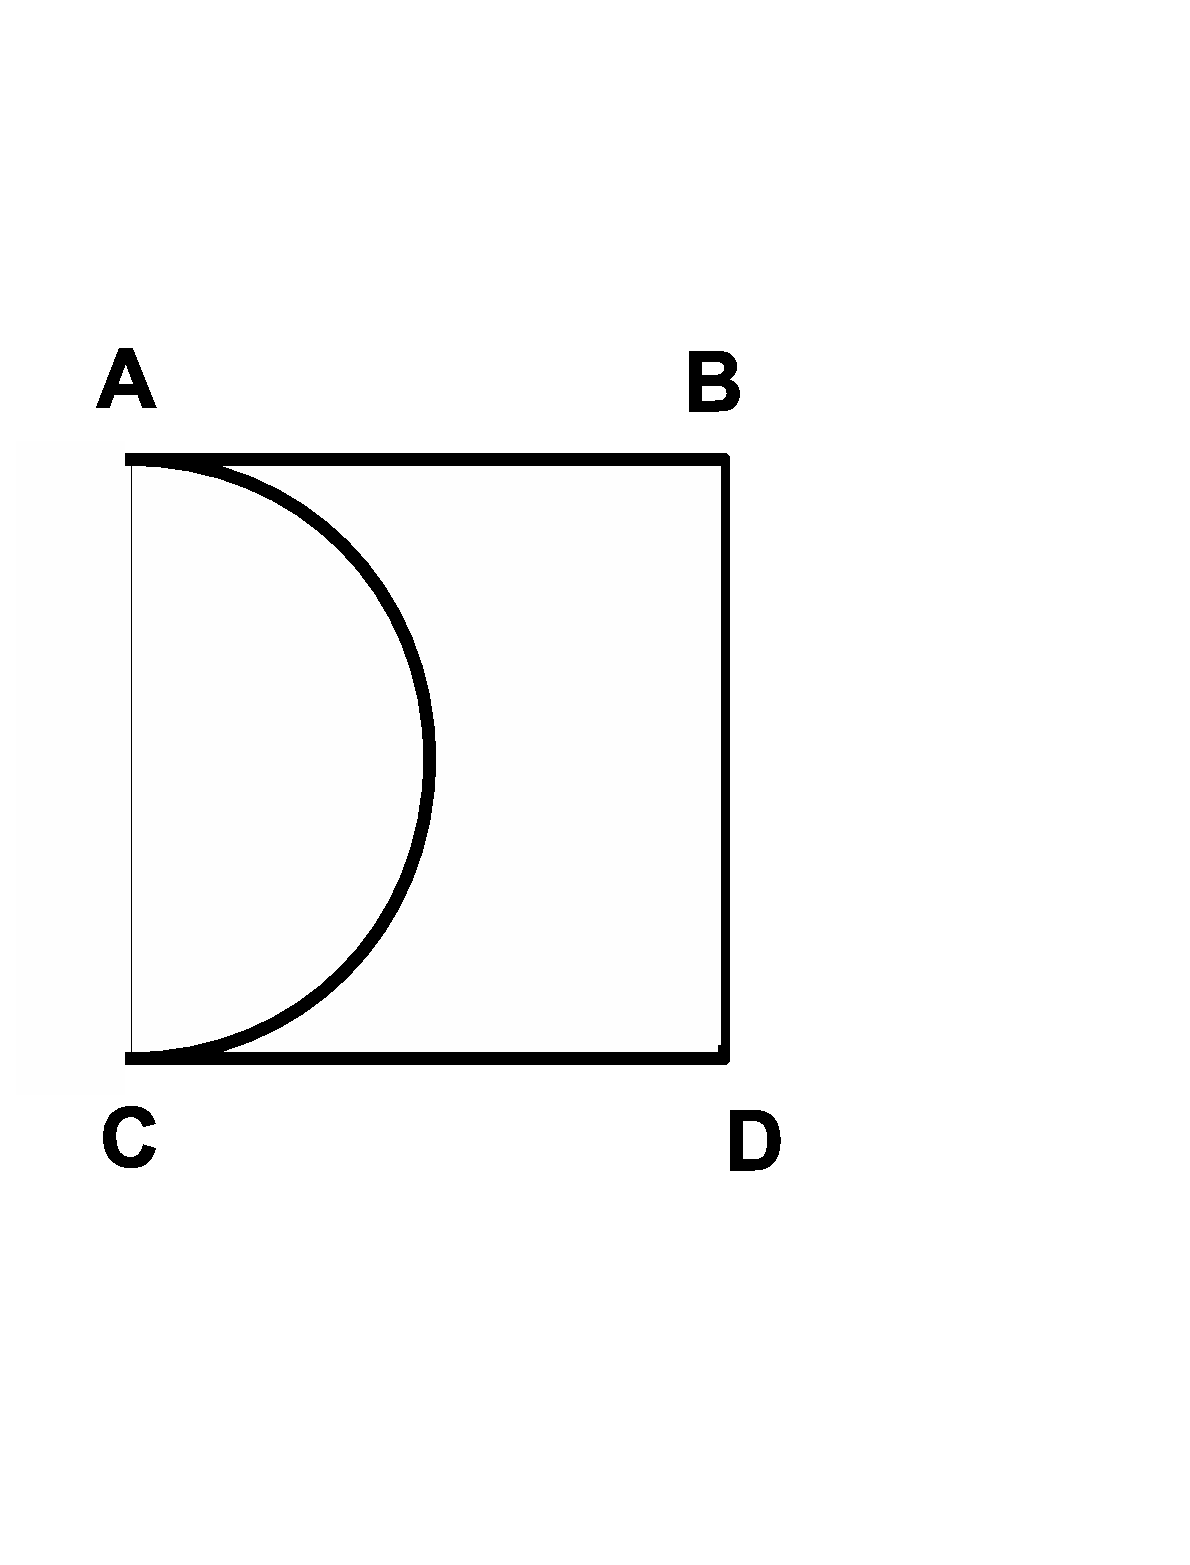
\includegraphics[width=30mm,viewport=22 180 351 579]{CCJPR74-4pic2.eps}
\end{wrapfigure}

\textbf{The correct answer is (E): 64}\\
Imagine the semi-circular area to the right of BD moved into the semi-circular gap to the right of AC. An $8\times8$ rectangle will have been formed. The area of the new region (which is equal to the area of the old region) is then $8\time8=64$.
%End
\\[5 ex]
%Begin
%Language English
%Source Cariboo College High School Mathematics competition
%Title Junior Preliminary Round 1974
%Question 5
%Subject arithmetic
%Category integers
%Type MC
%Choices 5
%Answer E
%Creator Victor Semenoff
%Rdifficulty 23
%Qtext

\scriptsize
Source: Cariboo College High School Mathematics Contest

\normalsize
%\begin{wrapfigure}[2]{r}[0pt]{0pt}
%	\includegraphics[width=30mm]{CCJ78-04}
%\end{wrapfigure}
$A$ and $B$ are both two-digit numbers with $A$ smaller than $B$. The set of numbers between, but not including, $A$ and $B$ contains 13 odd numbers and 14 even numbers. If the sum of $A$ and $B$ is 126, then $A$ equals:\\
%ChoiceA
(A) 77\\
%ChoiceB
(B) 76\\
%ChoiceC
(C) 63\\
%ChoiceD
(D) 50\\
%ChoiceE
(E) 49\\
%Ftext

%\begin{wrapfigure}{r}[0pt]{0pt}
%	\includegraphics[width=30mm]{CCJ78-04}
%\end{wrapfigure}

\textbf{The correct answer is (E): 49}\\
$B$ will be the $13+14+1=28^{\textrm{th}}$ number after $A$. Thus $B=A+28$. Since the sum of $A$ and $B$ is 126, we have
\begin{align*}
A+(A+28)&=126\\
2A&=126-28=98\\
A&=49.
\end{align*}
%End
\\[5 ex]
%Begin
%Language English
%Source Cariboo College High School Mathematics competition
%Title Junior Preliminary Round 1974
%Question 6
%Subject statistics
%Category concepts
%Type MC
%Choices 5
%Answer A
%Creator Victor Semenoff
%Rdifficulty 21
%Qtext

\scriptsize
Source: Cariboo College High School Mathematics Contest

\normalsize
%\begin{wrapfigure}[4]{r}[0pt]{0pt}
%	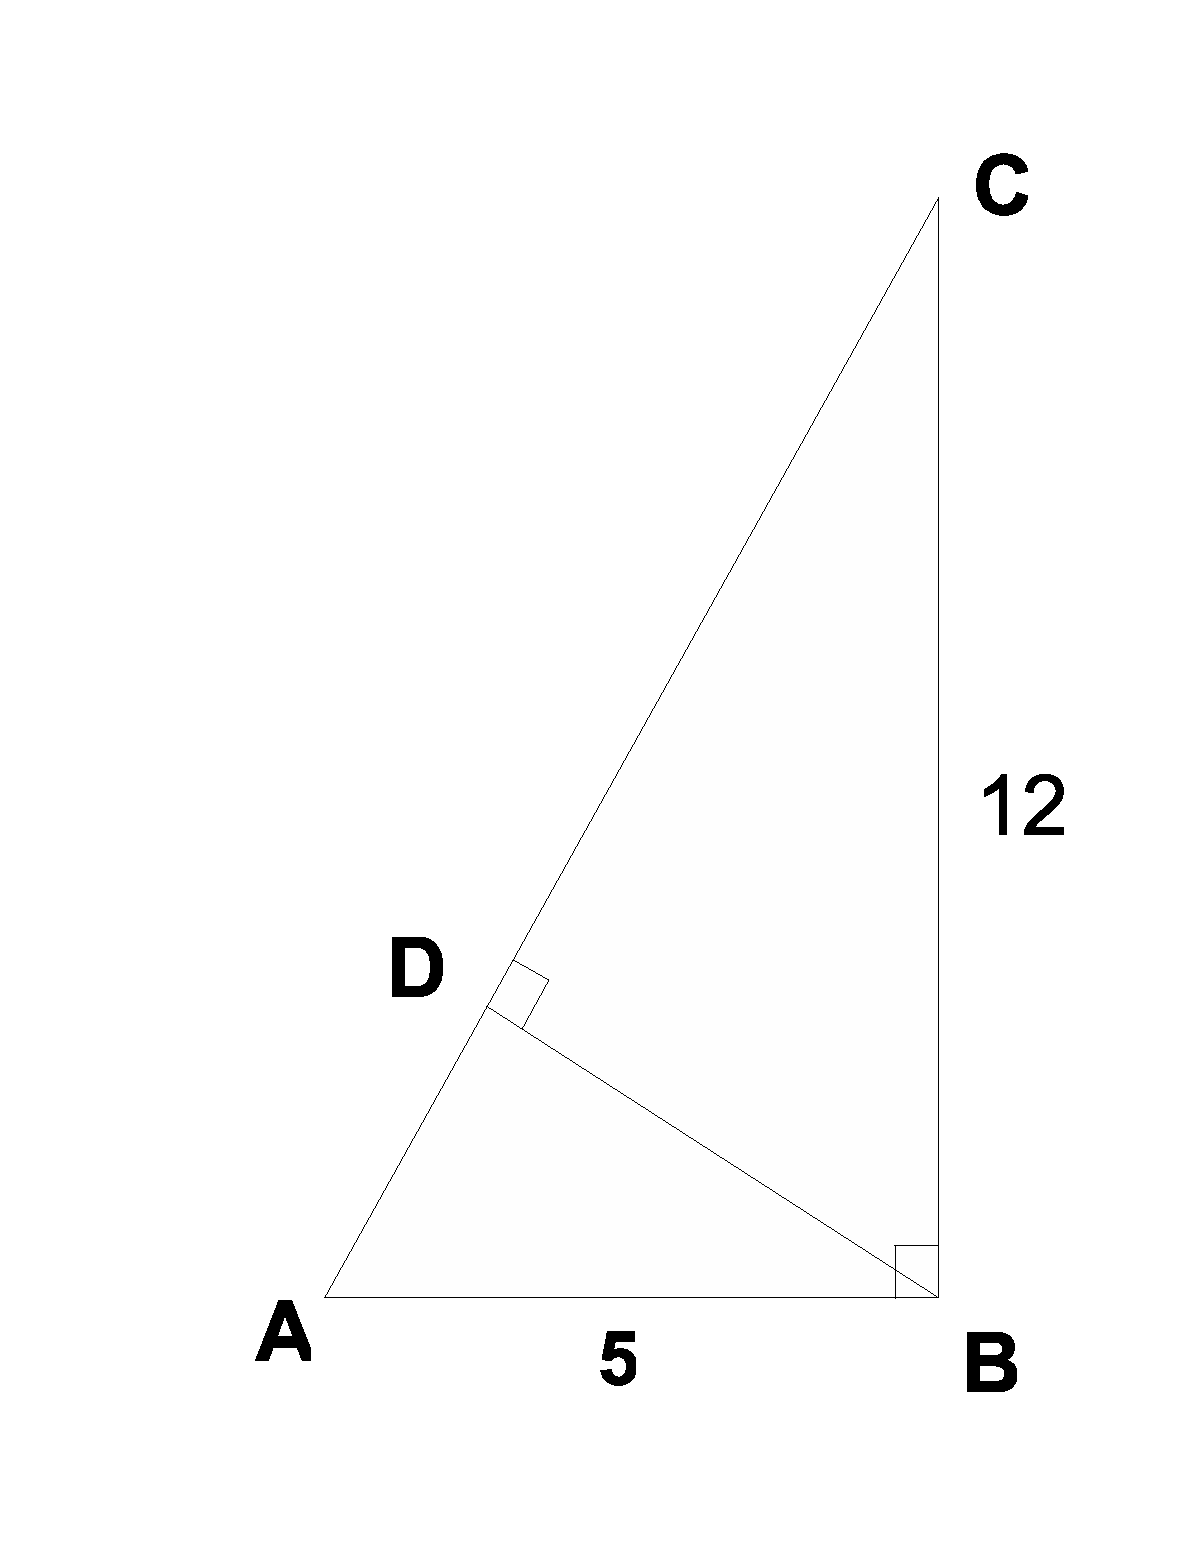
\includegraphics[width=25mm,viewport=100 67 508 675]{CCSPR73-6pic.eps}
%\end{wrapfigure}
A group of boys and girls consists of 20 boys and 20 girls. How many girls must be added to the group so that the resulting group will be $60\%$ girls?\\
%ChoiceA
(A) 10\\
%ChoiceB
(B) 20\\
%ChoiceC
(C) 40\\
%ChoiceD
(D) 90\\
%ChoiceE
(E) None of these.\\
%Ftext

%\begin{wrapfigure}{r}[0pt]{0pt}
%	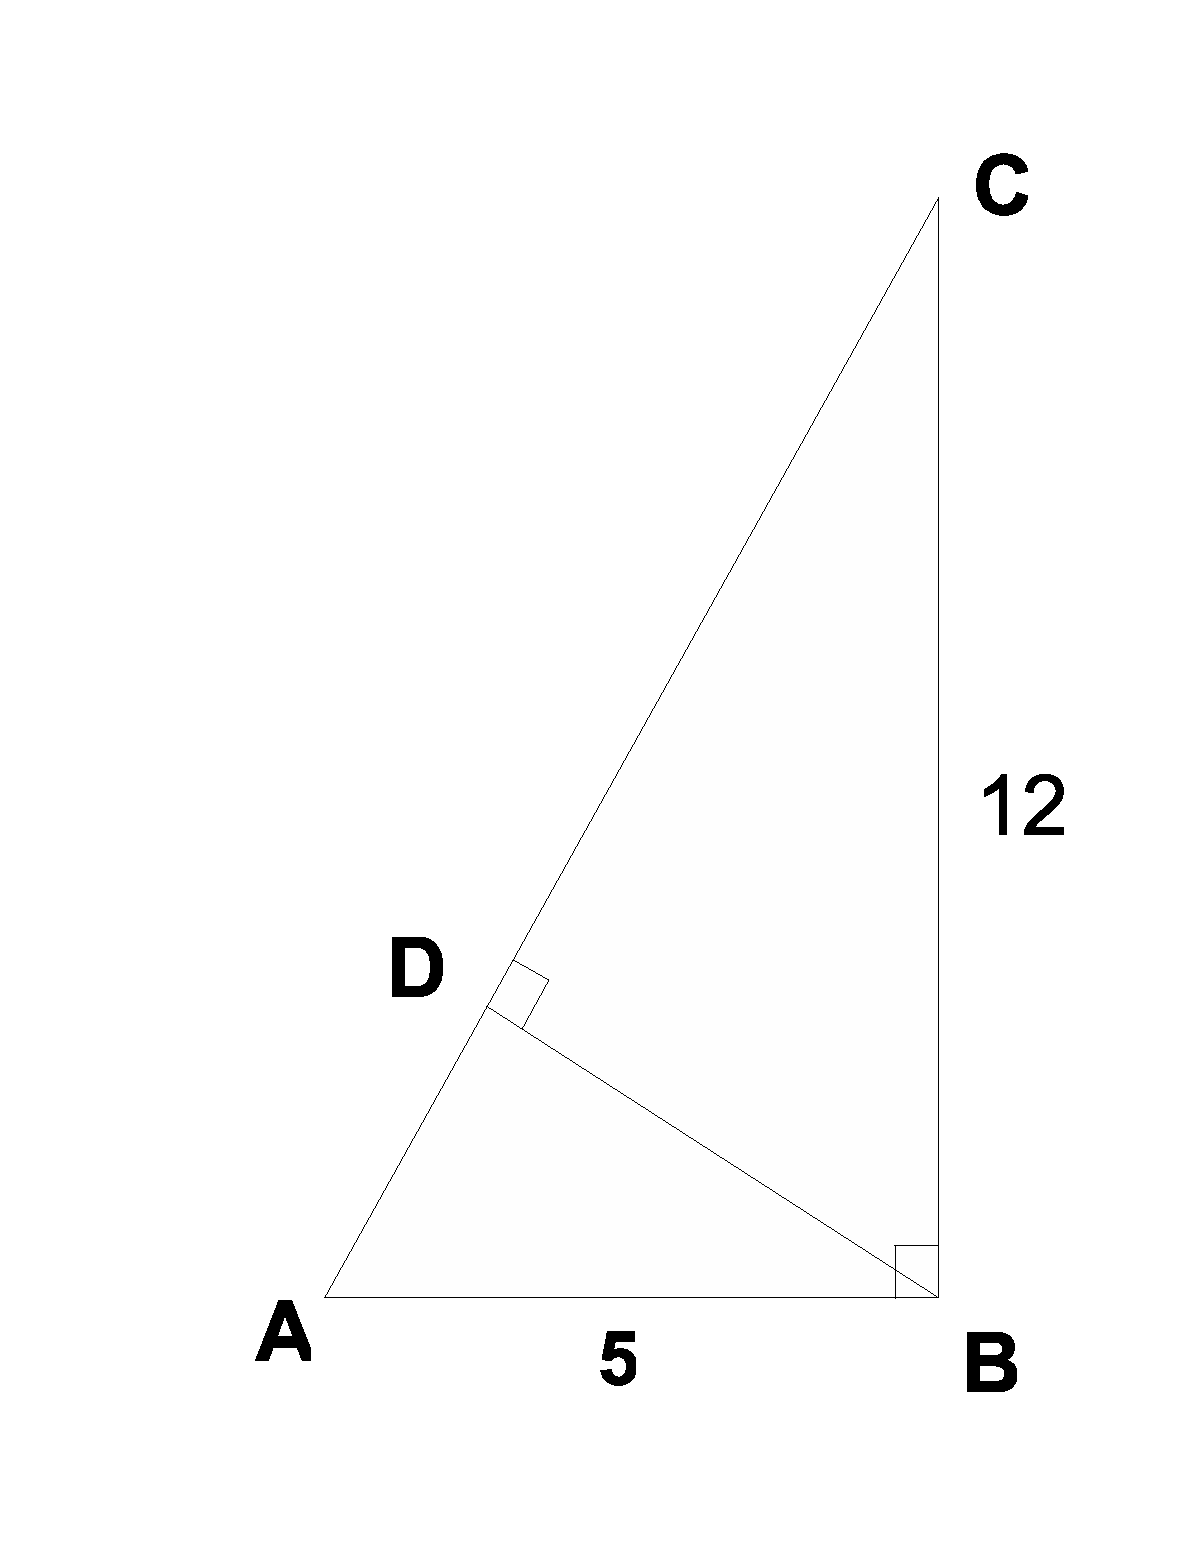
\includegraphics[width=25mm,viewport=100 67 508 675]{CCSPR73-6pic.eps}
%\end{wrapfigure}
\textbf{The correct answer is (A): 10}\\
Let $g$ be the number of girls that must be added to the group. After the girls are added, there will be 20+$g$ girls in the group and $40+g$ people. Since $60\%$ of the resulting group is to be girls, we require
\begin{equation*}
\frac{20+g}{40+g}=60\%
\end{equation*}
Solving for g we get
\begin{align*}
20+g=60\%(40+g)&=\frac{3}{5}(40+g)=24+\frac{3}{5}g\\
\frac{2}{5}g&=4\\
g&=49.
\end{align*}
%End
\\[5 ex]
%Begin
%Language English
%Source Cariboo College High School Mathematics competition
%Title Junior Preliminary Round 1974
%Question 7
%Subject geometry
%Category length
%Type MC
%Choices 5
%Answer D
%Creator Victor Semenoff
%Rdifficulty 23
%Qtext

\scriptsize
Source: Cariboo College High School Mathematics Contest

\normalsize
%\begin{wrapfigure}[2]{r}[0pt]{0pt}
%	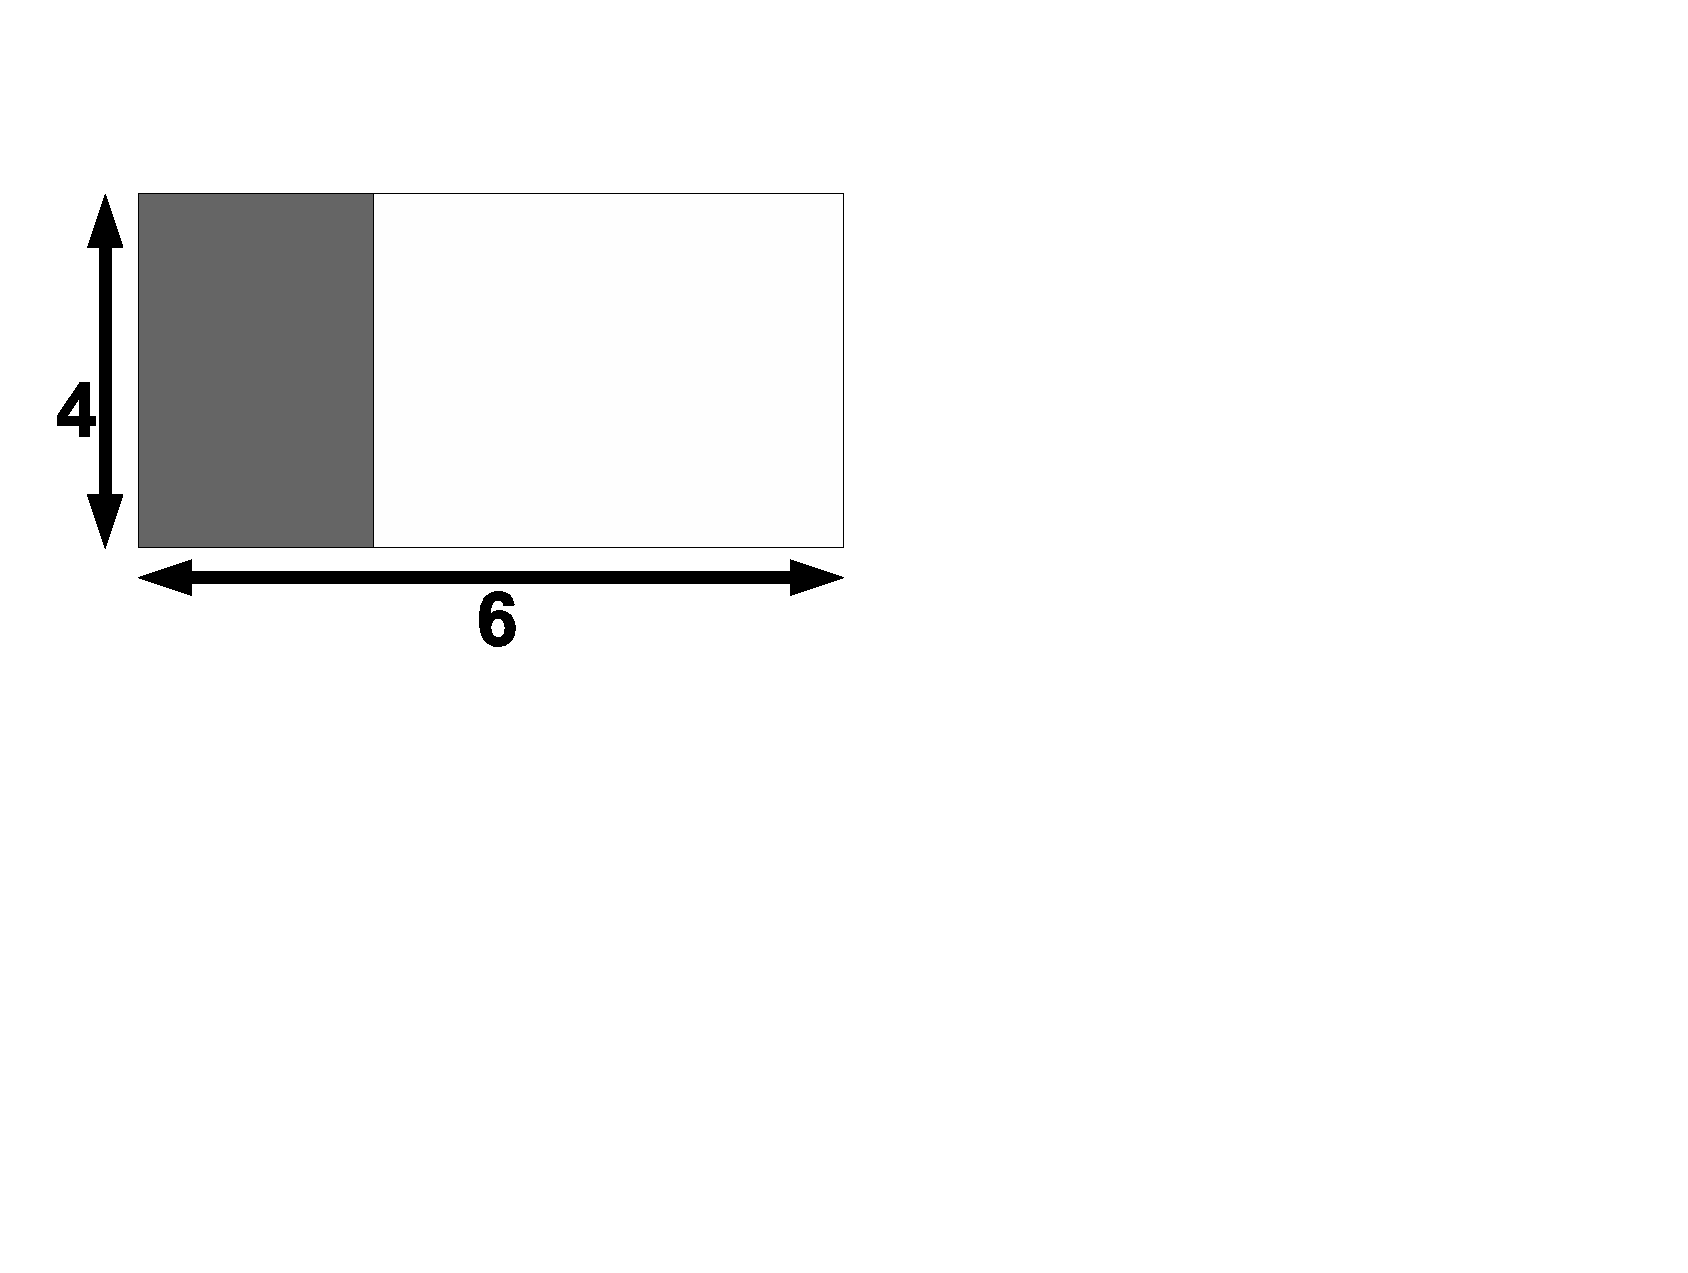
\includegraphics[width=30mm,viewport=17 290 402 516]{CCJPR73-7pic.eps}
%\end{wrapfigure}
The length of a rectangle is twice its width. If the area of the rectangle is $A$, and the perimeter is $P$ then $\frac{(A+P^{2})}{A}$ equals:\\
%ChoiceA
(A) 3\\
%ChoiceB
(B) 4\\
%ChoiceC
(C) 18\\
%ChoiceD
(D) 19\\
%ChoiceE
(E) None of these.\\
%Ftext

%\begin{wrapfigure}{r}[0pt]{0pt}
%	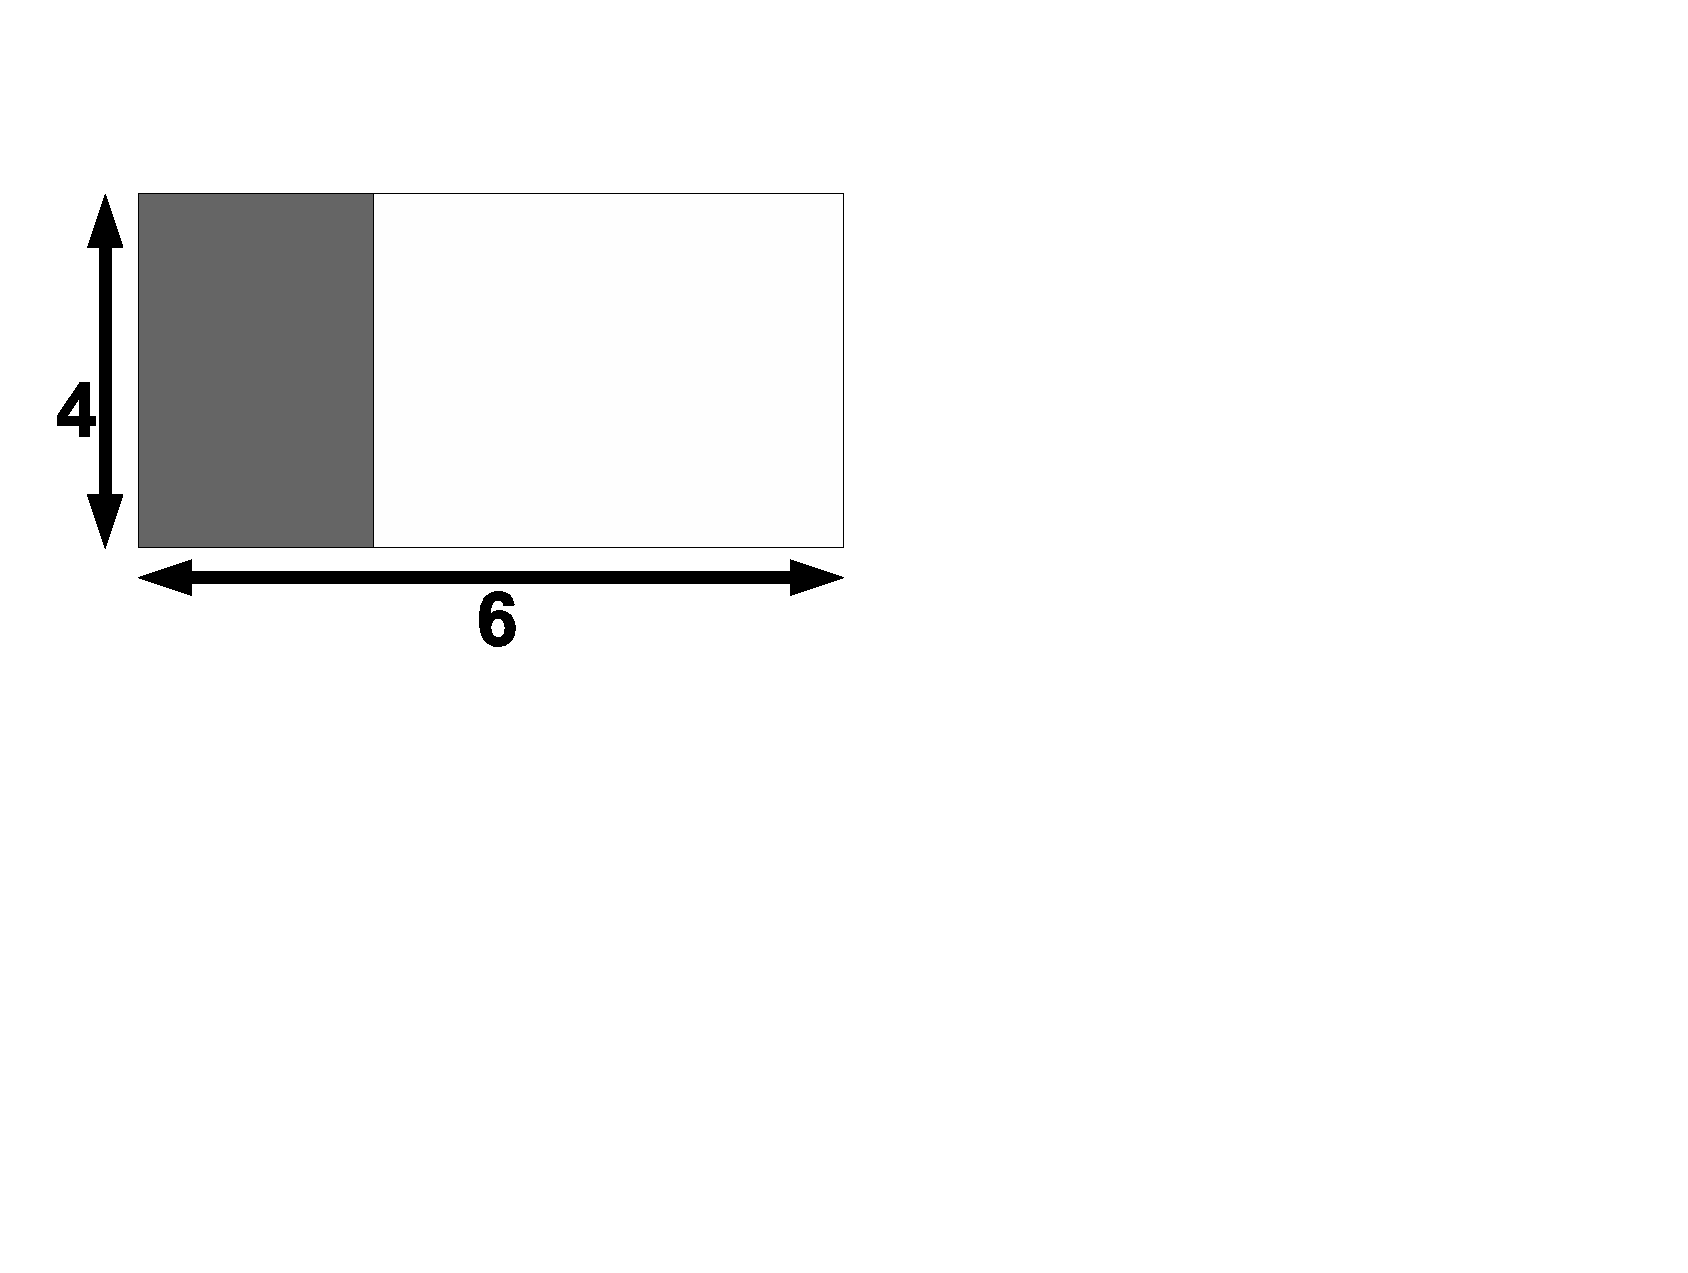
\includegraphics[width=30mm,viewport=17 290 402 516]{CCJPR73-7pic.eps}
%\end{wrapfigure}

\textbf{The correct answer is (D): 19}\\[1ex]
Let $w$ be the width of the rectangle, and let $l$ be its length. Since the rectangle is twice as long as it is wide, we have $l=2w$. Thus
\begin{equation*}
A=lw=2w^2.
\end{equation*}
And
\begin{equation*}
P=2(l+w)=2(2w+w)=6w.
\end{equation*}
Therefore
\begin{equation*}
\frac{A+P^{2}}{A}=\frac{2w^{2}+(6w)^{2}}{2w^{2}}=\frac{38w^{2}}{2w^{2}}=19.
\end{equation*}
%End
\\[5 ex]
%Begin
%Language English
%Source Cariboo College High School Mathematics competition
%Title Junior Preliminary Round 1974
%Question 8
%Subject geometry
%Category area
%Type MC
%Choices 5
%Answer E
%Creator Victor Semenoff
%Rdifficulty 27
%Qtext

\scriptsize
Source: Cariboo College High School Mathematics Contest

\normalsize
\begin{wrapfigure}[2]{r}[0pt]{0pt}
	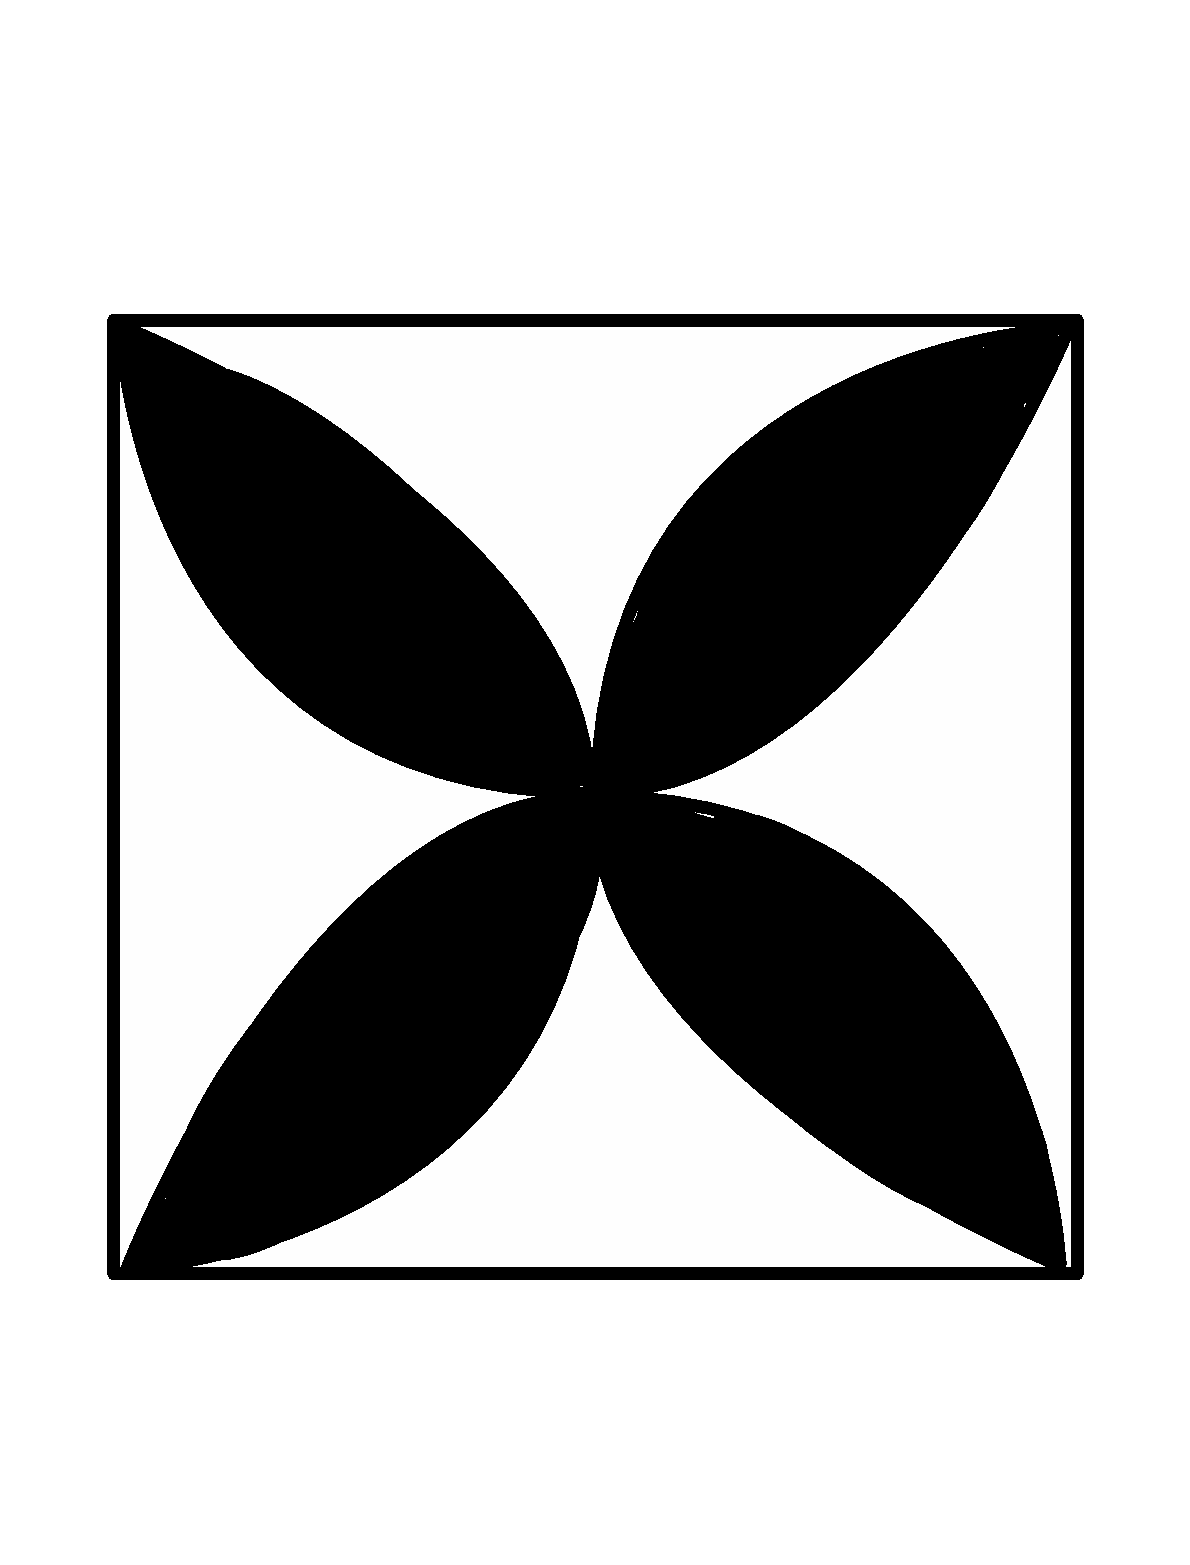
\includegraphics[width=30mm,viewport=36 122 514 596]{CCJPR74-8pic.eps}
\end{wrapfigure}
The figure is made up from intersecting \textbf{semi}-circles of diameter 12. The area of the shaded region is:\\
%ChoiceA
(A) 48\\
%ChoiceB
(B) 21\\
%ChoiceC
(C) $18(\pi-1)$\\
%ChoiceD
(D) $36(4-\pi)$\\
%ChoiceE
(E) None of these.\\
%Ftext

\begin{wrapfigure}{r}[0pt]{0pt}
	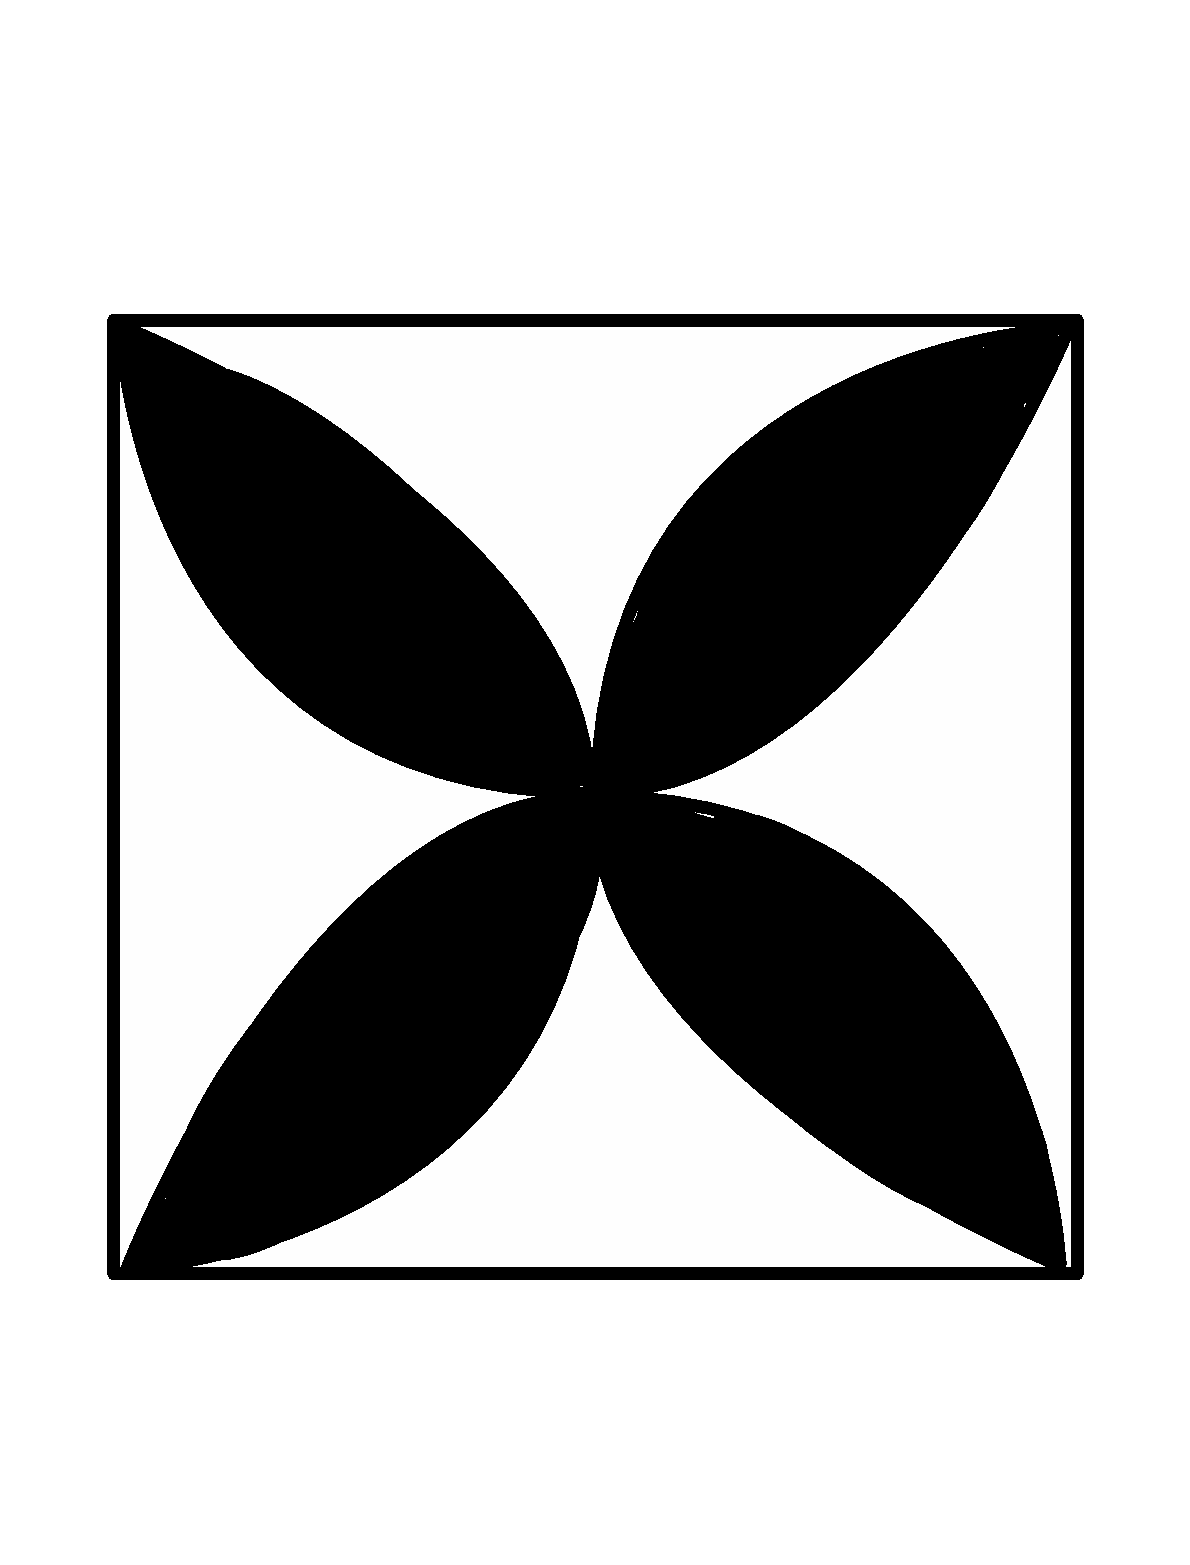
\includegraphics[width=30mm,viewport=36 122 514 596]{CCJPR74-8pic.eps}
\end{wrapfigure}

\textbf{The correct answer is (E): None of these.}\\[1 ex]
Let $A_{sq}$ be the area of the square, $A_{sc}$ the area of the semi-circles, and $A_{sh}$ the area of the shaded region. We know that $4A_{sc}=A_{sq}+A_{sh}$ because we will have counted each semi-circle twice. Since the diameter of each semi-circle is 12, its radius will be 6, and hence its area will be $A_{sc}=\frac{1}{2}\times\pi6^2$. Since the length of the sides of the square is equal to the diameter of the circles, $A_{sq}=12\times12$. Putting it all together we have
\begin{equation*}
A_{sh}=4(\frac{1}{2}\pi36)-12\times12=72(\pi-2).
\end{equation*}
%End
\\[5 ex]
%Begin
%Language English
%Source Cariboo College High School Mathematics competition
%Title Junior Preliminary Round 1974
%Question 9
%Subject geometry
%Category area
%Type MC
%Choices 5
%Answer D
%Creator Victor Semenoff
%Rdifficulty 22
%Qtext

\scriptsize
Source: Cariboo College High School Mathematics Contest

\normalsize
%\begin{wrapfigure}[2]{r}[0pt]{0pt}
%	\includegraphics[width=30mm,viewport=]{CCJ78-04}
%\end{wrapfigure}
A girl has a square sheet of paper which measures 64cm by 64cm. She cuts the square in half and discards one of the pieces. She then cuts the remaining piece in half and discards one of the pieces. She repeats this process until she has discarded ten pieces of paper. The area (in cm$^{2}$) of the paper she has left is:\\
%ChoiceA
(A) 409.6\\
%ChoiceB
(B) 8\\
%ChoiceC
(C) 6.4\\
%ChoiceD
(D) 4\\
%ChoiceE
(E) 2\\
%Ftext

%\begin{wrapfigure}{r}[0pt]{0pt}
%	\includegraphics[width=30mm,viewport=]{CCJ78-04}
%\end{wrapfigure}

\textbf{The correct answer is (D): 4}\\[1 ex]
The area of the $1^{st}$ square is 
\begin{equation*}
64\times64=2^{6}\times2^{6}=2^{12}
\end{equation*}
Each cut divides the remaining area by 2, and 10 cuts are made, thus the remaining area after 10 cuts is
\begin{equation*}
\frac{2^{12}}{2^{10}}=2^{2}=4.
\end{equation*}
%End
\\[5 ex]
%Begin
%Language English
%Source Cariboo College High School Mathematics competition
%Title Junior Preliminary Round 1974
%Question 10
%Subject functions
%Category rational
%Type MC
%Choices 5
%Answer B
%Creator Victor Semenoff
%Rdifficulty 22
%Qtext

\scriptsize
Source: Cariboo College High School Mathematics Contest

\normalsize
%\begin{wrapfigure}[4]{r}[0pt]{0pt}
%	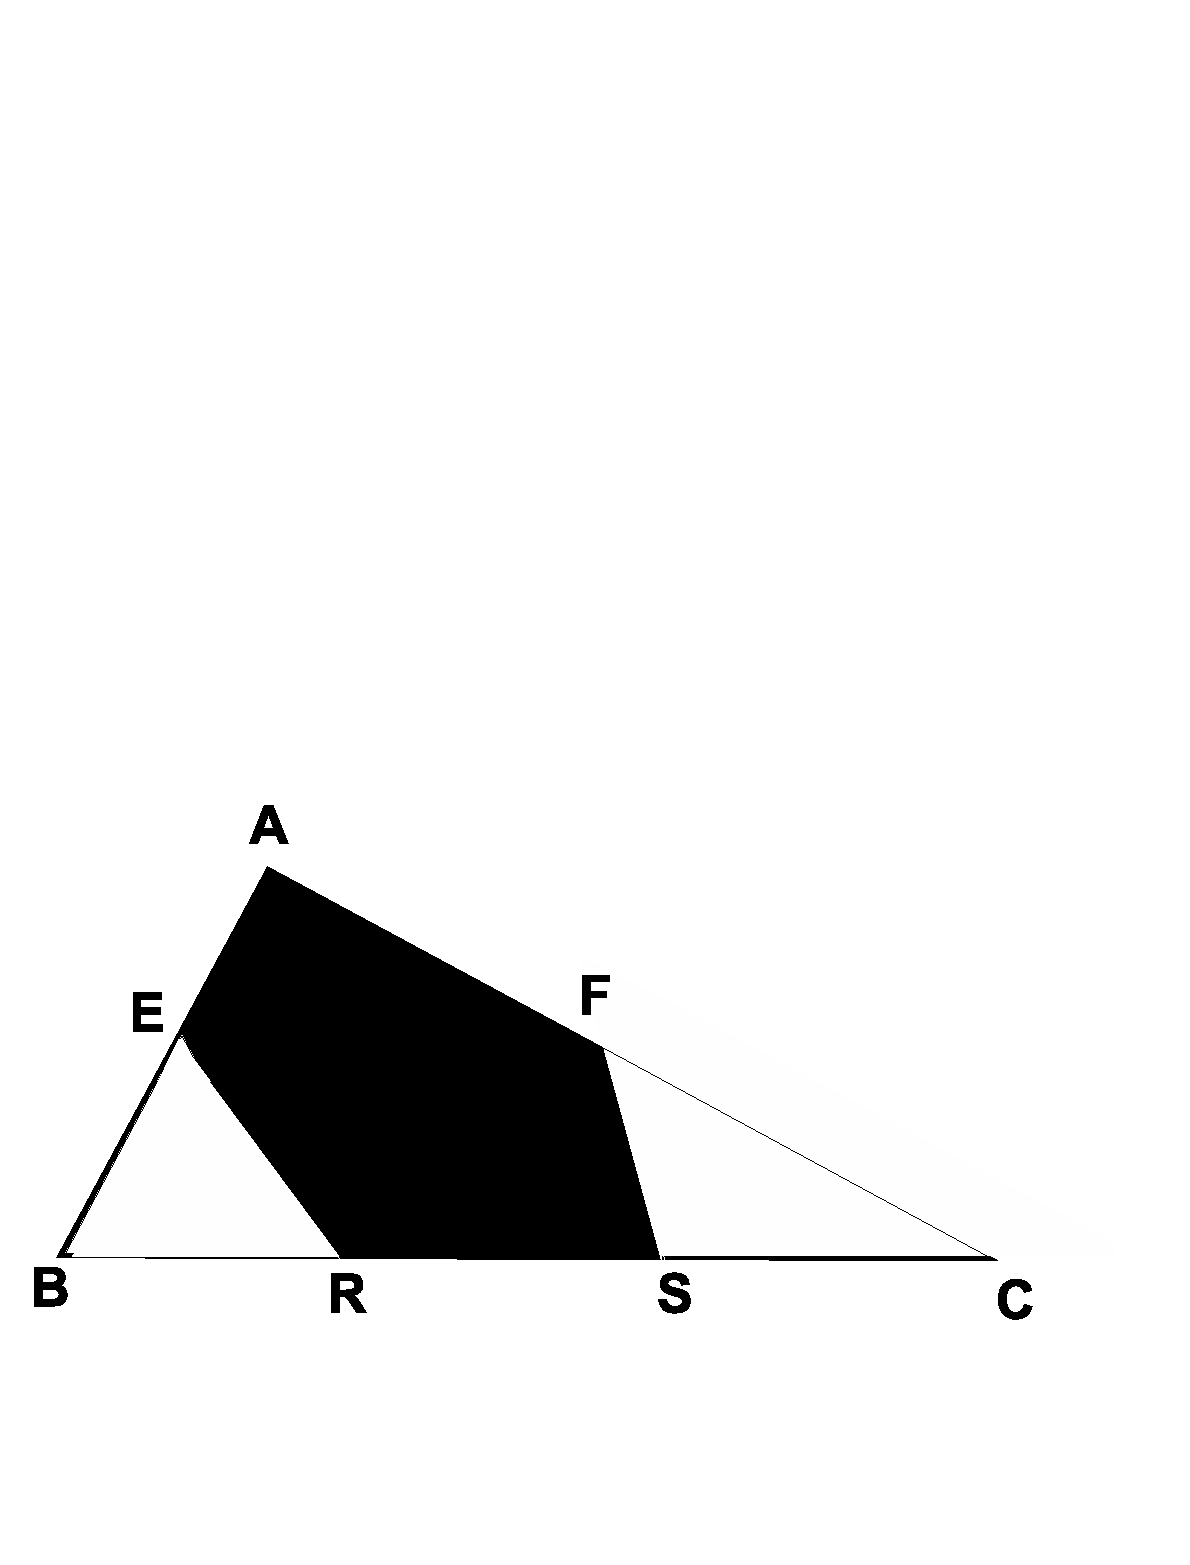
\includegraphics[width=35mm,viewport=4 102 497 362]{CCSPR73-10pic.eps}
%\end{wrapfigure}
If $\frac{x+y}{x-y}=\frac{3}{5}$, then $\frac{x}{y}$ equals:\\
%ChoiceA
(A) 5\\
%ChoiceB
(B) $-4$\\
%ChoiceC
(C) 3\\
%ChoiceD
(D) $\frac{5}{3}$\\
%ChoiceE
(E) None of these.\\
%Ftext\\

%\begin{wrapfigure}{r}[0pt]{0pt}
%	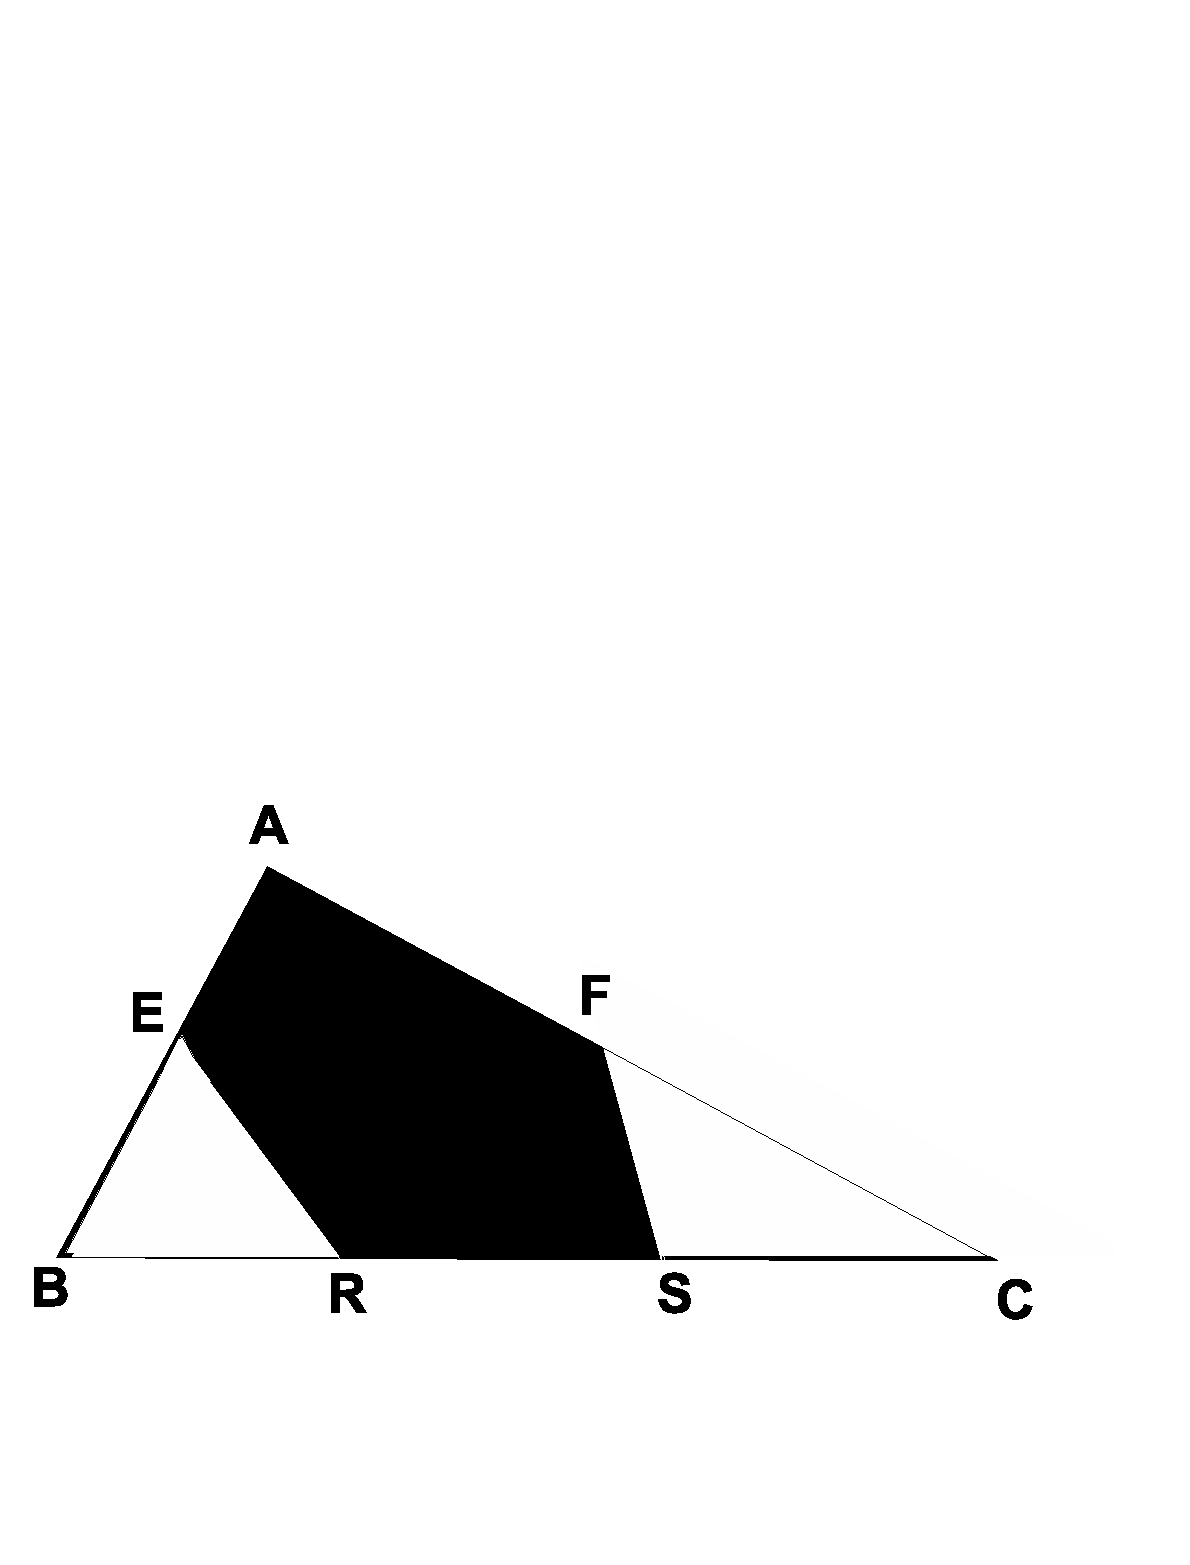
\includegraphics[width=35mm,viewport=4 102 497 362]{CCSPR73-10pic.eps}
%\end{wrapfigure}

\textbf{The correct answer is (B): $-4$}\\[1 ex]
\begin{align*}
\frac{x+y}{x-y}&=\frac{3}{5}\\
5x+5y&=3x-3y\\
2x&=-8y\\
\frac{x}{y}=-4.
\end{align*}
%End
\\[5 ex]
%Begin
%Language English
%Source Cariboo College High School Mathematics competition
%Title Junior Preliminary Round 1974
%Question 11
%Subject geometry
%Category area
%Type MC
%Choices 5
%Answer B
%Creator Victor Semenoff
%Rdifficulty 27
%Qtext

\scriptsize
Source: Cariboo College High School Mathematics Contest

\normalsize
\begin{wrapfigure}[4]{r}[0pt]{0pt}
	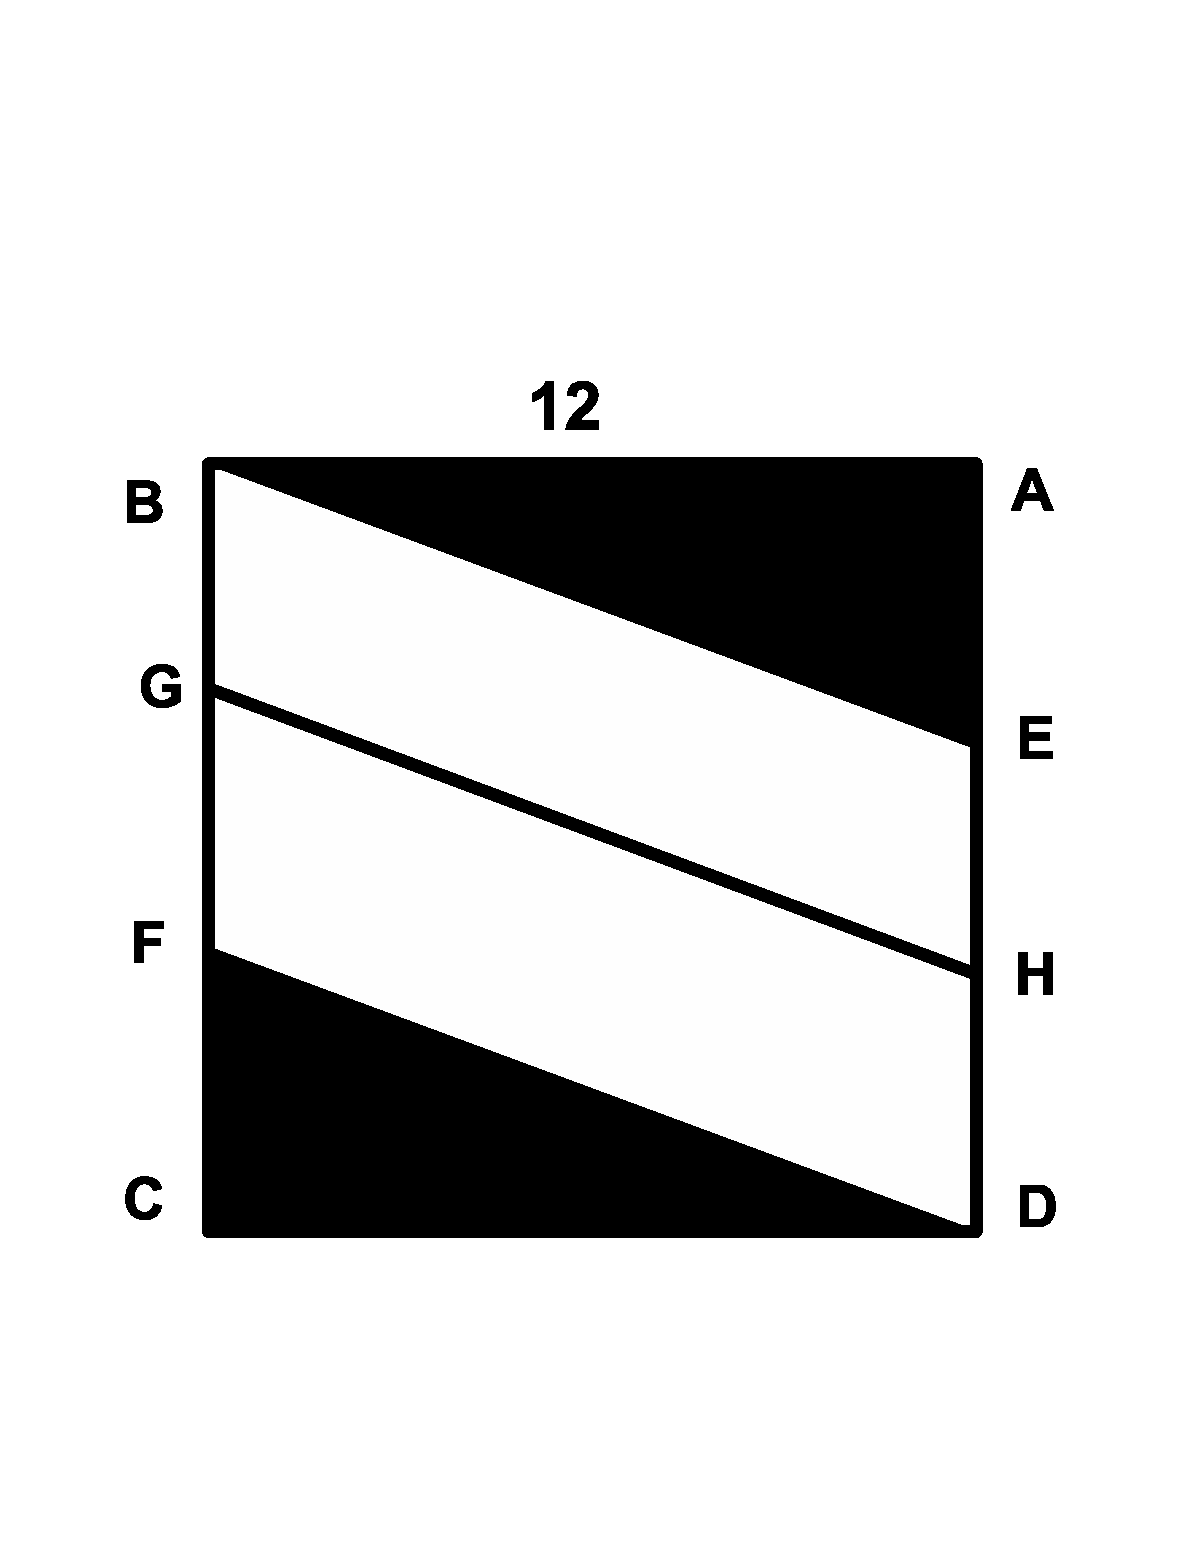
\includegraphics[width=30mm,viewport=44 173 501 563]{CCJPR74-11pic.eps}
\end{wrapfigure}
ABCD is a square, $\triangle$ABE and $\triangle$CDF are congruent, G and H are the mid-points of FB and DE respectively, and AB=12. If the unshaded portion is $\frac{7}{12}$ the area of ABCD, how long is HG?\\
%ChoiceA
(A) $\sqrt{193}$\\
%ChoiceB
(B) 13\\
%ChoiceC
(C) 15\\
%ChoiceD
(D) $2\sqrt{85}$\\
%ChoiceE
(E) None of these.\\
%Ftext

\begin{wrapfigure}{r}[0pt]{0pt}
	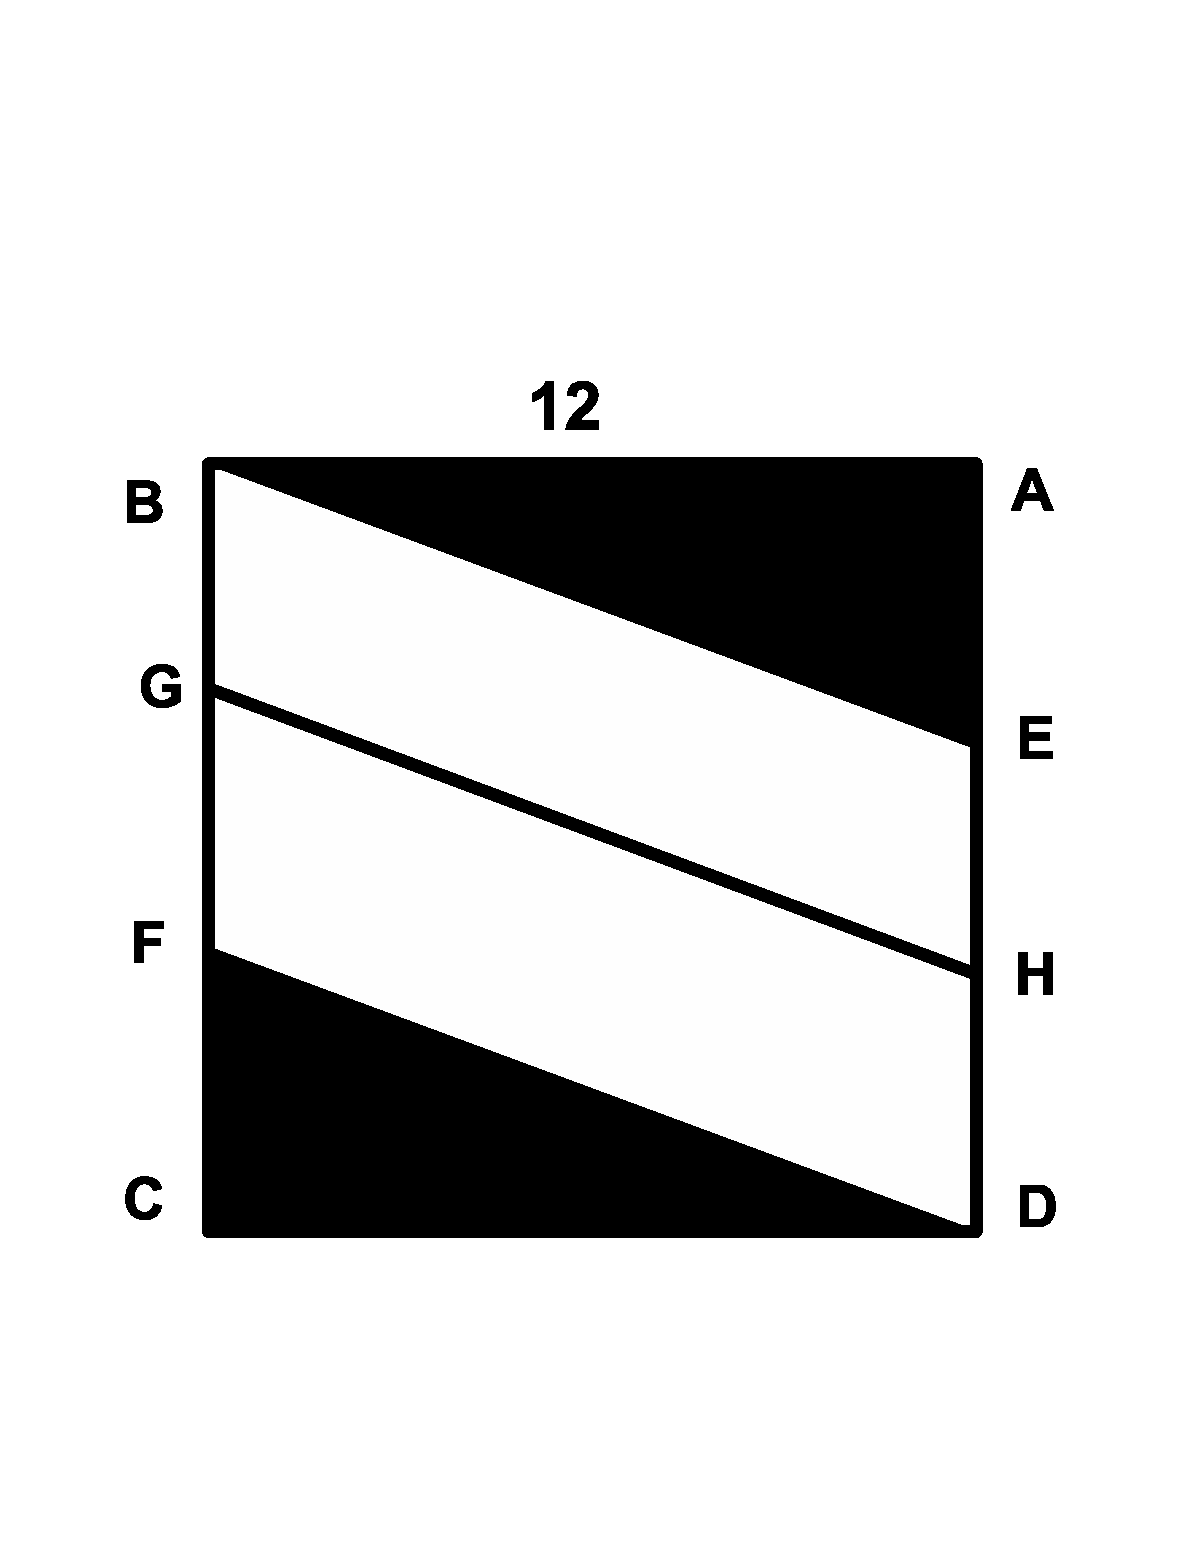
\includegraphics[width=30mm,viewport=44 173 501 563]{CCJPR74-11pic.eps}
\end{wrapfigure}

\textbf{The correct answer is (B): 13}\\[1 ex]
Since $\triangle$ABE and $\triangle$CDF are congruent, FC=AE. Thus BF=ED, and FD must be parallel to BE. Also, since BF=ED, and G and H are the respective midpoints of these two segments, BG=EH, and HG must be parallel to EB. Therefore, the unshaded region in the square is a parallelogram. If we let AB be the altitude of this parallelogram, its base will be ED=12-AE. The area of the parallelogram will then be ED$\times12$=(12-AE)$\times12$. Since we are told this is $\frac{7}{12}$ the area of ABCD, and we know that the area of ABCD is $12\times12$, we have
\begin{align*}
(12-\textrm{AE})\times12&=\frac{7}{12}12\times12=7\times12\\
\textrm{AE}&=5
\end{align*}
Since $\triangle$ABE is a right triangle, and AB=12, while AE=5, EB must be 13. Since HG is parallel to EB, its length is also 13.
%End
\\[5 ex]
%Begin
%Language English
%Source Cariboo College High School Mathematics competition
%Title Junior Preliminary Round 1974
%Question 12
%Subject geometry
%Category area
%Type MC
%Choices 5
%Answer E
%Creator Victor Semenoff
%Rdifficulty 28
%Qtext

\scriptsize
Source: Cariboo College High School Mathematics Contest

\normalsize
%\begin{wrapfigure}[2]{r}[0pt]{0pt}
%	\includegraphics[width=30mm,viewport=]{CCJ78-04}
%\end{wrapfigure}
A circular running track $w$ feet wide has the same area as a circle with radius $5w$. The inside length of the track is:\\
%ChoiceA
(A) $8w$\\
%ChoiceB
(B) $13\pi w$\\
%ChoiceC
(C) $12w$\\
%ChoiceD
(D) $25\pi w$\\
%ChoiceE
(E) $24\pi w$\\
%Ftext

%\begin{wrapfigure}{r}[0pt]{0pt}
%	\includegraphics[width=30mm,viewport=]{CCJ78-04}
%\end{wrapfigure}

\textbf{The correct answer is (E): $24\pi w$}\\[1 ex]
Let $r$ be the distance from the centre of the track to the inside of the track. The distance from the centre of the track to the outside of the track will then be $r+w$. The track will thus have an area equal to the area of a circle with radius $r+w$ minus the area of the circle with radius $r$, or
\begin{equation*}
\pi(r+w)^{2}-\pi r^{2}=\pi(r^{2}+2wr+w^{2}-r^{2})=\pi(2wr+w^{2})
\end{equation*}
The area of the circle with radius $5w$ is $\pi25w^2$. Since this is to be equal to the area of the track, we have the equation
\begin{align*}
\pi25w^{2}&=\pi(2wr+w^{2})\\
2wr&=24w^{2}\\
r&=12w
\end{align*}
Since the distance from the centre of the race track to the inside of the track is 12w, the inside length of the the track will be $2\pi(12w)=24\pi w$.
%End
\\[5 ex]
%Begin
%Language English
%Source Cariboo College High School Mathematics competition
%Title Junior Preliminary Round 1974
%Question 13
%Subject statistics
%Category concepts
%Type MC
%Choices 5
%Answer B
%Creator Victor Semenoff
%Rdifficulty 21
%Qtext

\scriptsize
Source: Cariboo College High School Mathematics Contest

\normalsize
%\begin{wrapfigure}[2]{r}[0pt]{0pt}
%	\includegraphics[width=30mm,viewport=]{CCJ78-04}
%\end{wrapfigure}
In the city of Xonia five percent of the population were eligible to vote in their recent election. As it turned out 7,000 women and 2,000 men voted; in all, three percent of the population. What is the maximum number of eligible male voters that there can possibly be?\\
%ChoiceA
(A) 10,000\\
%ChoiceB
(B) 8,000\\
%ChoiceC
(C) 7,000\\
%ChoiceD
(D) 15,000\\
%ChoiceE
(E) 17,000\\
%Ftext

%\begin{wrapfigure}{r}[0pt]{0pt}
%	\includegraphics[width=30mm,viewport=]{CCJ78-04}
%\end{wrapfigure}

\textbf{The correct answer is (B): 8,000}\\[1 ex]
Let $p$ be the population of Xonia, and let $v=7,000+2,000=9000$ be the total number voters. Since $5\%$ of the population were eligible, but only $3\%$ voted, then there were $\frac{2}{100}p$ citizens who coul vote but did not. Also, we know that
\begin{align*}
\frac{3}{100}p&=v\\
p&=\frac{100}{3}v
\end{align*}
The maximum number of males who could have voted will equal the number of males who voted, plus the number of males who were eligible but did not vote. The maximum occurs when all the non-voters who were eligible are males. Then the maximum number is
\begin{align*}
2,000+\frac{2}{100}p &=2,000+\frac{2}{3}v\\
2,000+\frac{2}{3}(9000)&=8,000.
\end{align*}
%End
\\[5 ex]
%Begin
%Language English
%Source Cariboo College High School Mathematics competition
%Title Junior Preliminary Round 1974
%Question 14
%Subject probability
%Category counting
%Type MC
%Choices 5
%Answer C
%Creator Victor Semenoff
%Rdifficulty 24
%Qtext

\scriptsize
Source: Cariboo College High School Mathematics Contest

\normalsize
%\begin{wrapfigure}[2]{r}[0pt]{0pt}
%	\includegraphics[width=30mm,viewport=]{CCJ78-04}
%\end{wrapfigure}
How many four-digit numbers with digits (from left to right) a, b, c, d have the property that if each of the digits is divided by 7 the remainders are 2, 1, 0, and 4, respectively?\\
%ChoiceA
(A) 1\\
%ChoiceB
(B) 4\\
%ChoiceC
(C) 8\\
%ChoiceD
(D) 16\\
%ChoiceE
(E) 9\\
%Ftext

%\begin{wrapfigure}{r}[0pt]{0pt}
%	\includegraphics[width=30mm,viewport=]{CCJ78-04}
%\end{wrapfigure}

\textbf{The correct answer is (C): 8}\\[1 ex]
The digit a can be 2 or 9, be can be 1 or 8, c can be 0 or 7, and d can be 4. Since the remainder when one digit is divided by 7 is independent of the remainder when the other digits are divided by 7, we have 2 choices for a, b, and c and 1 choice for d. Thus there are $2\times2\times2\times1=8$ numbers that have the stated property.
%End
\\[5 ex]
%Begin
%Language English
%Source Cariboo College High School Mathematics competition
%Title Junior Preliminary Round 1974
%Question 15
%Subject arithmetic
%Category integers
%Type MC
%Choices 5
%Answer D
%Creator Victor Semenoff
%Rdifficulty 23
%Qtext

\scriptsize
Source: Cariboo College High School Mathematics Contest

\normalsize
%\begin{wrapfigure}[2]{r}[0pt]{0pt}
%	\includegraphics[width=30mm,viewport=]{CCJ78-04}
%\end{wrapfigure}
Given the set of numbers \{8,16,24,...,1000\} and the set of numbers \{6,12,18,...,996\}, how many numbers belong to both sets?\\
%ChoiceA
(A) 20\\
%ChoiceB
(B) 21\\
%ChoiceC
(C) 40\\
%ChoiceD
(D) 41\\
%ChoiceE
(E) 42\\
%Ftext

%\begin{wrapfigure}{r}[0pt]{0pt}
%	\includegraphics[width=30mm,viewport=]{CCJ78-04}
%\end{wrapfigure}

\textbf{The correct answer is (D): 41}\\[1 ex]
The numbers in the first set are the multiples of 8 less than or equal to 1000, while the numbers in the second set are the multiples of 6 less than or equal to 996. Since $8=2^3$ and $6=2\times3$, numbers that are multiples of $2^{3}\times3=24$ and are less that 996 will appear in both sets.

These numbers can be represented by $24n$, where $n$ is an integer. Since we require $24n\leq996$, we get $n\leq41.5$. And because $n$ is an integer, there will be 41 such numbers.
%End
\\[5 ex]
%Begin
%Language English
%Source Cariboo College High School Mathematics competition
%Title Junior Preliminary Round 1974
%Question 16
%Subject geometry
%Category length
%Type MC
%Choices 5
%Answer A
%Creator Victor Semenoff
%Rdifficulty 24
%Qtext

\scriptsize
Source: Cariboo College High School Mathematics Contest

\normalsize
\begin{wrapfigure}[4]{r}[0pt]{0pt}
	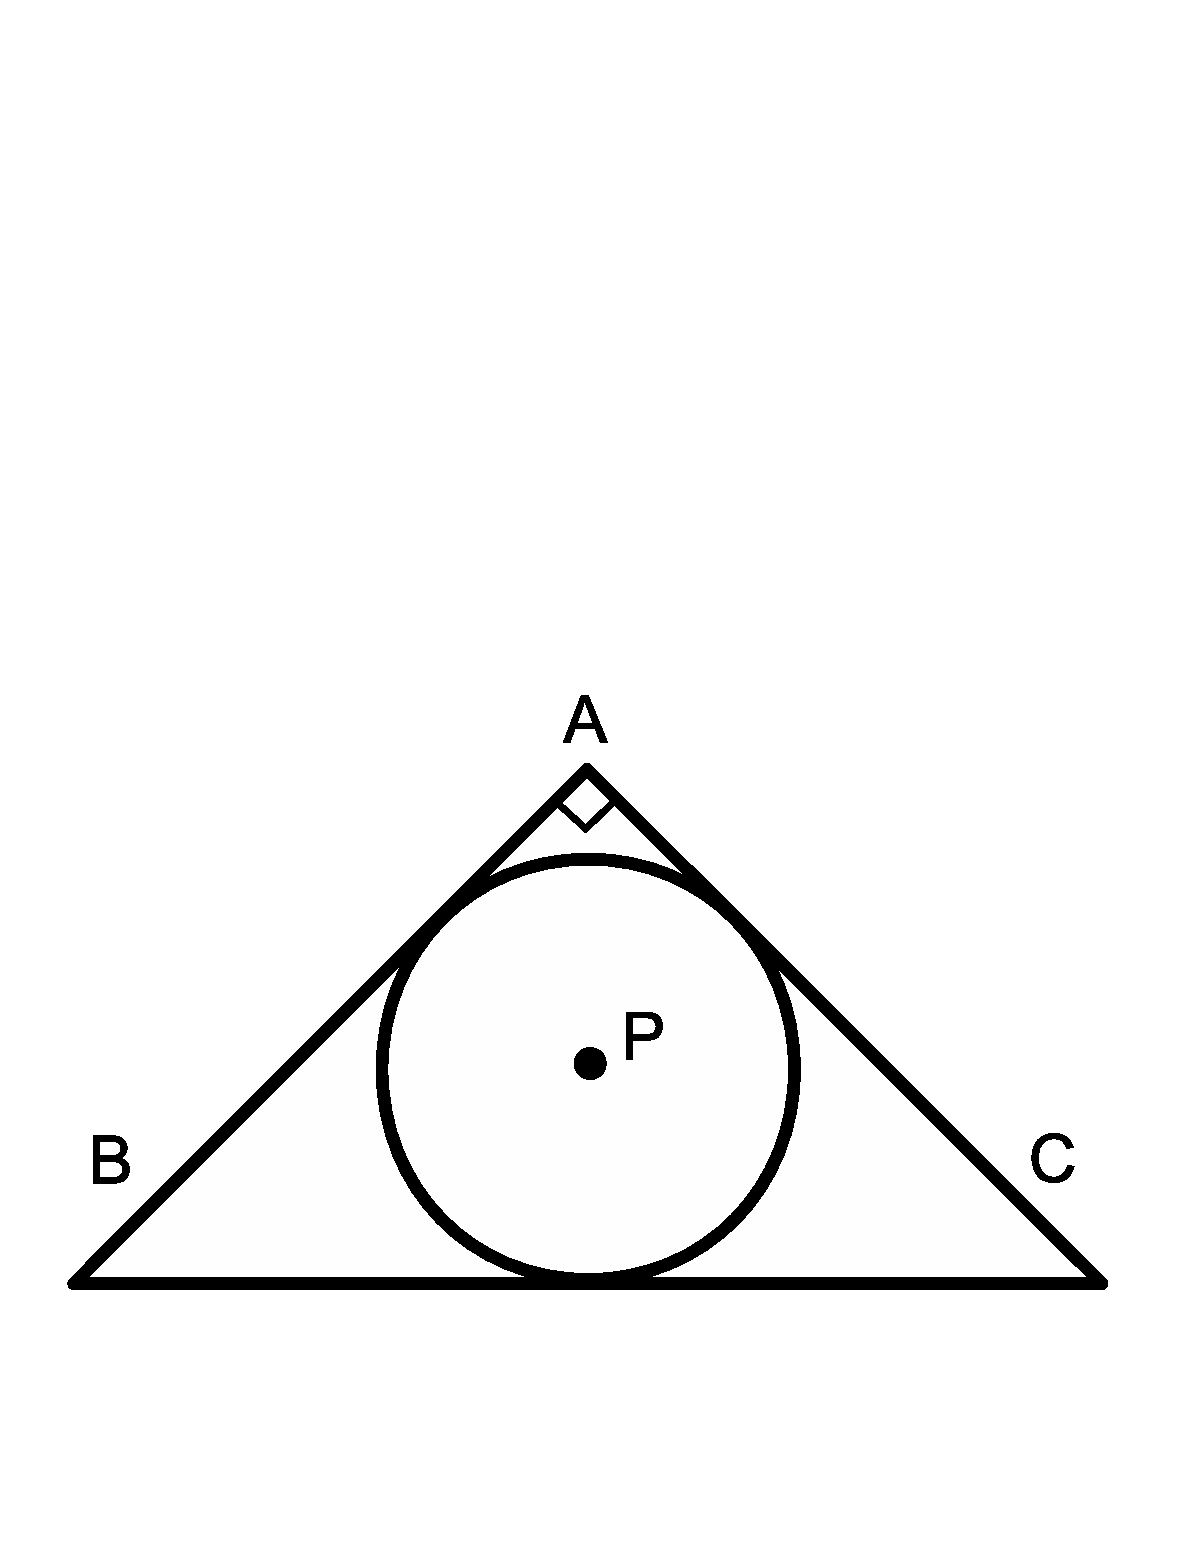
\includegraphics[width=30mm,viewport=19 116 527 413]{CCJPR74-16pic.eps}
\end{wrapfigure}
In the right triangle shown AB=AC=12 and P is the centre of the inscribed circle. The radius of the inscribed circle is:\\
%ChoiceA
(A) $12-6\sqrt{2}$\\
%ChoiceB
(B) $6\sqrt{2}-6$\\
%ChoiceC
(C) 4\\
%ChoiceD
(D) $2\sqrt{6}$\\
%ChoiceE
(E) 3\\
%Ftext

\begin{wrapfigure}{r}[0pt]{0pt}
	\includegraphics[width=30mm,viewport=16 83 534 412]{CCJPR74-16pic2.eps}
\end{wrapfigure}

\textbf{The correct answer is (A): $12-6\sqrt{2}$}\\[1 ex]
Let $r$ be the radius of the circle, and let AX be a segment perpendicular to BC. Since $\angle$ACB=$45^{\circ}$ and AC=12, we see that AX=$\frac{12}{\sqrt{2}}=6\sqrt{2}$ If a radius of the circle is drawn to AC, a $45^{\circ}$-$45^{\circ}$-$90^{\circ}$ triangle, this hypotenuse will also equal $r\sqrt{2}$. Thus we have
\begin{align*}
6\sqrt{2}-r&=r\sqrt{2}\\
r(\sqrt{2}+1)&=6\sqrt{2}\\
r=\frac{6\sqrt{2}}{\sqrt{2}+1}&=\frac{6\sqrt{2}}{\sqrt{2}+1}\times\frac{\sqrt{2}-1}{\sqrt{2}-1}=\frac{6\times2-6\sqrt{2}}{2-1}=12-6\sqrt{2}.
\end{align*}
%End
\\[5 ex]
%Begin
%Language English
%Source Cariboo College High School Mathematics competition
%Title Junior Preliminary Round 1974
%Question 17
%Subject arithmetic
%Category integers
%Type MC
%Choices 5
%Answer E
%Creator Victor Semenoff
%Rdifficulty 23
%Qtext

\scriptsize
Source: Cariboo College High School Mathematics Contest

\normalsize
%\begin{wrapfigure}[2]{r}[0pt]{0pt}
%	\includegraphics[width=30mm,viewport=]{CCJ78-04}
%\end{wrapfigure}
Given the sequence \{11,18,25,32,39,...\}, a new sequence is formed by subtracting 3 from each term. Which one of the following numbers appears in the new sequence?\\
%ChoiceA
(A) 221\\
%ChoiceB
(B) 222\\
%ChoiceC
(C) 223\\
%ChoiceD
(D) 224\\
%ChoiceE
(E) 225\\
%Ftext

%\begin{wrapfigure}{r}[0pt]{0pt}
%	\includegraphics[width=30mm,viewport=]{CCJ78-04}
%\end{wrapfigure}

\textbf{The correct answer is (E): 225\\}\\[1 ex]
The terms in the old series can be represented by $11+7n$, where $n$ is an integer. If 3 is subtracted from each term in the old series, the terms in the new series can be represented by
\begin{equation*}
11+7n-3=8+7n,
\end{equation*}
where n is the same as before. For a number $m$ to appear in this new series there must be some integer $n$ such that $8+7n=m$. This will be possible if $\frac{m-8}{7}$ is an integer, which of the choices given only occurs for 225.
%End
\\[5 ex]
%Begin
%Language English
%Source Cariboo College High School Mathematics competition
%Title Junior Preliminary Round 1974
%Question 18
%Subject algebra
%Category modelling
%Type MC
%Choices 5
%Answer D
%Creator Victor Semenoff
%Rdifficulty 28
%Qtext

\scriptsize
Source: Cariboo College High School Mathematics Contest

\normalsize
%\begin{wrapfigure}[2]{r}[0pt]{0pt}
%	\includegraphics[width=30mm,viewport=]{CCJ78-04}
%\end{wrapfigure}
Three cars travel at constant speeds over a long, straight track. If they start at the same time at the same end of the track, we find that car A finishes the track when B has 120 meters to go, and C has 210 meters to go to get to the finish. When car B finishes, car C has 100 meters to go to reach the finish. The length of the track (in meters) is:\\
%ChoiceA
(A) 1000\\
%ChoiceB
(B) 1050\\
%ChoiceC
(C) 1100\\
%ChoiceD
(D) 1200\\
%ChoiceE
(E) Not enough information.\\
%Ftext

%\begin{wrapfigure}{r}[0pt]{0pt}
%	\includegraphics[width=30mm,viewport=]{CCJ78-04}
%\end{wrapfigure}

\textbf{The correct answer is (D): 1200}\\[1 ex]
Let $l$ be the length of the track in meters. When A crosses the line, B has traveled $l-120$ and C has traveled $l-210$. Thus the ratio of the distance B has traveled to that of C is
\begin{equation}
l-120:l-210.
\end{equation}
When car B crosses the line, it has traveled $l$ and C has traveled $l-100$. The ratio of the distances is then
\begin{equation}
l:l-100
\end{equation}
Since the cars travel at constant speeds, we can equate the ratios in (1) and (2).
\begin{align*}
l-120:l-210&=l:l-100\\
\frac{l-120}{l-210}&=\frac{l}{l-100}\\
(l-120)(l-100)&=l^{2}-l\times210\\
10l&=120\times100\\
l&=1200.
\end{align*}
%End
\\[5 ex]
%Begin
%Language English
%Source Cariboo College High School Mathematics competition
%Title Junior Preliminary Round 1974
%Question 19
%Subject algebra
%Category modelling
%Type MC
%Choices 5
%Answer B
%Creator Victor Semenoff
%Rdifficulty 27
%Qtext

\scriptsize
Source: Cariboo College High School Mathematics Contest

\normalsize
%\begin{wrapfigure}[2]{r}[0pt]{0pt}
%	\includegraphics[width=30mm,viewport=]{CCJ78-04}
%\end{wrapfigure}
On the Xonian temperature scale (measured in $X$ degrees) water freezes at $120^{\circ}X$ and boils at $12^{\circ}X$. When the temperature is $93^{\circ}X$ what is the temperature in degrees centigrade?\\
%ChoiceA
(A) -25\\
%ChoiceB
(B) 25\\
%ChoiceC
(C) -19\\
%ChoiceD
(D) 19\\
%ChoiceE
(E) 20\\
%Ftext

%\begin{wrapfigure}{r}[0pt]{0pt}
%	\includegraphics[width=30mm,viewport=]{CCJ78-04}
%\end{wrapfigure}

\textbf{The correct answer is (B): 25}\\[1 ex]
The difference between the boiling and freezing point of water on the Xonian temperature scale is $12^{\circ}X-120^{\circ}X=-108^{\circ}X$, while the difference between the boiling and freezing point of water on the Celsius scale is $100^{\circ}C$. When the temperature is $93^{\circ}X$, it is $93^{\circ}X-120^{\circ}X=-27^{\circ}X$ above freezing. This is
\begin{equation*}
\frac{-27^{\circ}X}{-108^{\circ}X}=\frac{1}{4}
\end{equation*}
of the way to the boiling point. The temperature on the Celsius scale will also be $\frac{1}{4}$ of the way from the freezing to the boiling point, or $\frac{1}{4}(100^{\circ}C)=25^{\circ}C$.
%End
\\[5 ex]
%Begin
%Language English
%Source Cariboo College High School Mathematics competition
%Title Junior Preliminary Round 1974
%Question 20 Part A
%Subject geometry
%Category area
%Type MC
%Choices 5
%Answer E
%Creator Victor Semenoff
%Rdifficulty 22
%Qtext

\scriptsize
Source: Cariboo College High School Mathematics Contest

\normalsize
\begin{wrapfigure}[7]{r}[0pt]{0pt}
	\includegraphics[width=25mm,viewport=66 28 464 700]{CCJPR74-20pic2.eps}
\end{wrapfigure}
The two squares ABCD and EFGH shown are each 4 by 4. If the first square is divided into 4 equal parts as shown and a circle is inscribed in each part, while the second square is divided into 16 equal parts, and a circle is inscribed in each of these parts, then the ratio of the total area of all the circles in the second square to the total area of all the circles in the first square is:\\
%ChoiceA
(A) 3:1\\
%ChoiceB
(B) $\pi$:1\\
%ChoiceC
(C) 2:1\\
%ChoiceD
(D) 3:2\\
%ChoiceE
(E) 1:1\\
%Ftext

\begin{wrapfigure}{r}[0pt]{0pt}
	\includegraphics[width=20mm,viewport=66 28 464 700]{CCJPR74-20pic2.eps}
\end{wrapfigure}

\textbf{The correct answer is (E): 1:1}\\[1 ex]
Let $D$ be the diameter of the large circle. The diameter of the small circle will then be $\frac{D}{2}$. Since the area of each large circle is
\begin{equation*}
\pi(\frac{D}{2})^2=\frac{\pi D^{2}}{4},
\end{equation*}
and there are 4 of them, the total area of all 4 is $\pi D^2$. The area of the small circle is
\begin{equation*}
\pi(\frac{\frac{D}{2}}{2})^2=\frac{\pi D^{2}}{16},
\end{equation*}
and there are 16 of them, so the total area of the small circles is $16\times\frac{\pi D^{2}}{16}=\pi D^2$. Thus the ratio of the total area of the large circles to the total area of the small circles is 1:1.
%End
\\[5 ex]
%Begin
%Language English
%Source Cariboo College High School Mathematics competition
%Title Junior Preliminary Round 1974
%Question 20 Part B
%Subject geometry
%Category area
%Type MC
%Choices 5
%Answer A
%Creator Victor Semenoff
%Rdifficulty 15
%Qtext

\scriptsize
Adapted From: Cariboo College High School Mathematics Contest

\normalsize
\begin{wrapfigure}[7]{r}[0pt]{0pt}
	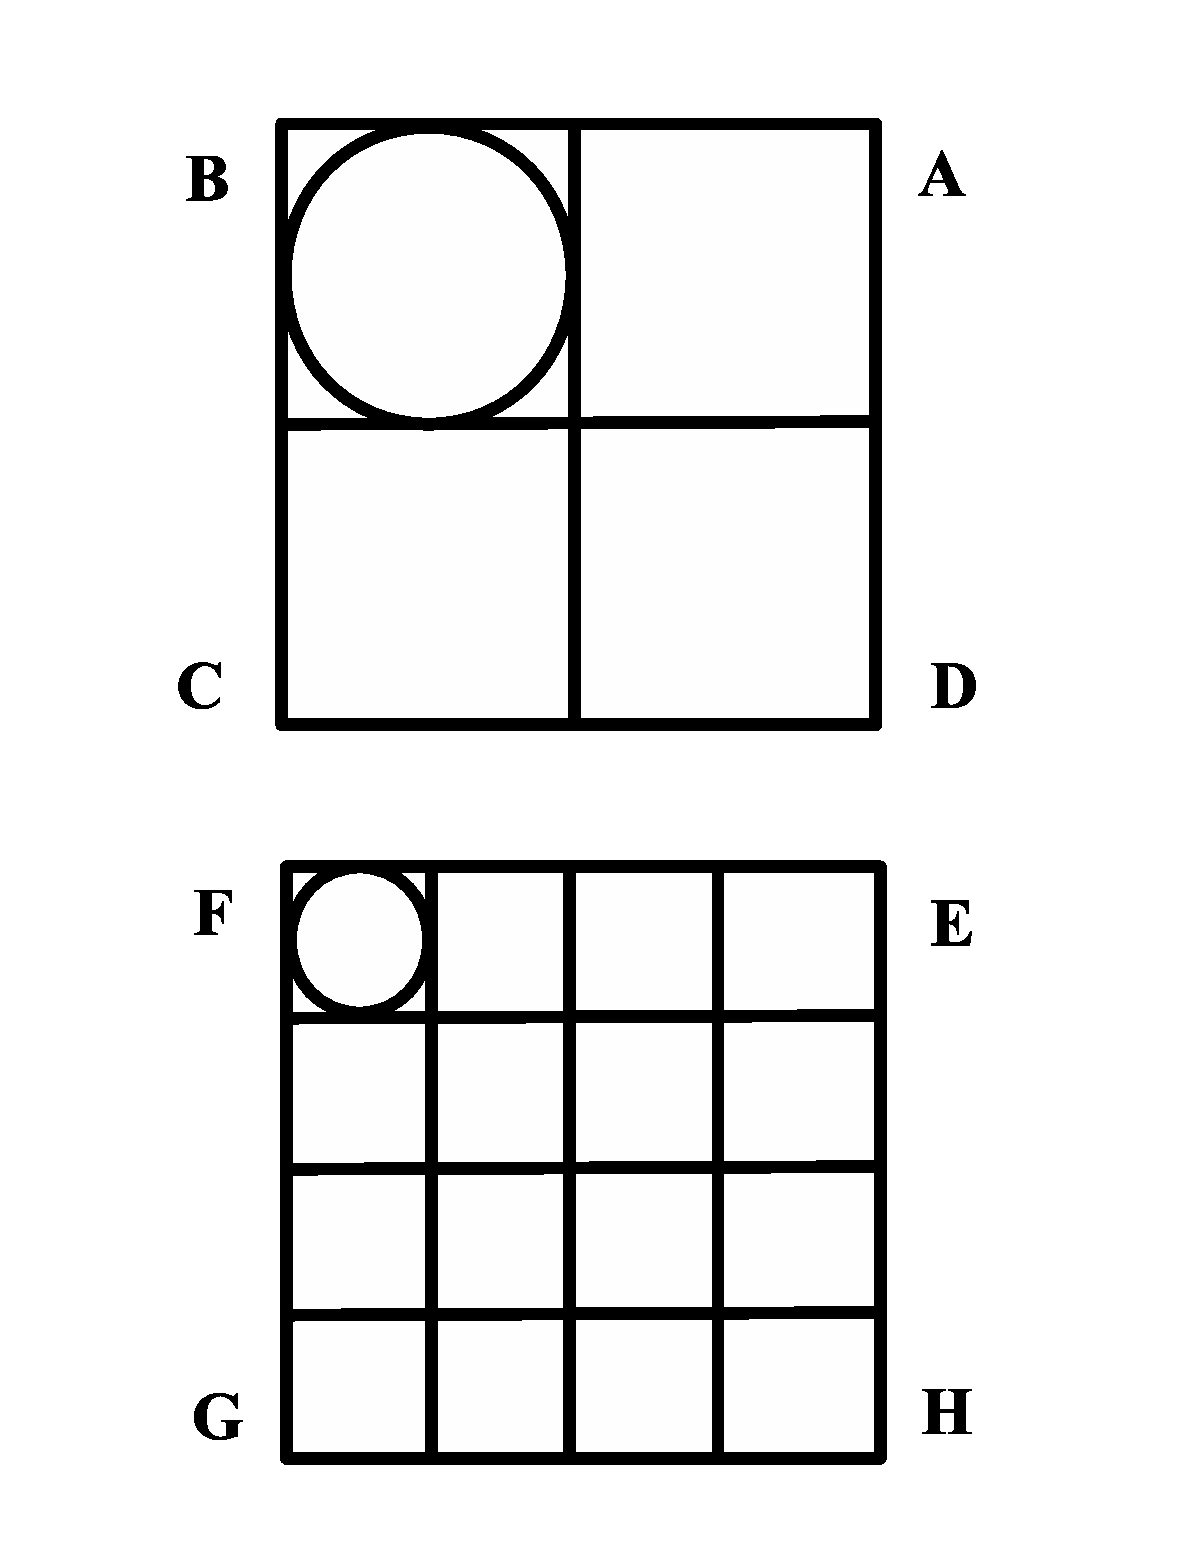
\includegraphics[width=25mm,viewport=66 28 464 700]{CCJPR74-20pic.eps}
\end{wrapfigure}
The two squares ABCD and EFGH shown are each 4 by 4. If the first square is divided into 4 equal parts as shown and a circle is inscribed in the top left section, while the second square is divided into 16 equal parts, and a circle is inscribed in the top left section, then the ratio of the area of the large circle to the area of the small circle is:\\
%ChoiceA
(A) 4:1\\[1 ex]
%ChoiceB
(B) $\pi$:1\\[1 ex]
%ChoiceC
(C) 3:1\\[1 ex]
%ChoiceD
(D) 2:1\\[1 ex]
%ChoiceE
(E) 3:2\\
%Ftext

\begin{wrapfigure}[7]{r}[0pt]{0pt}
	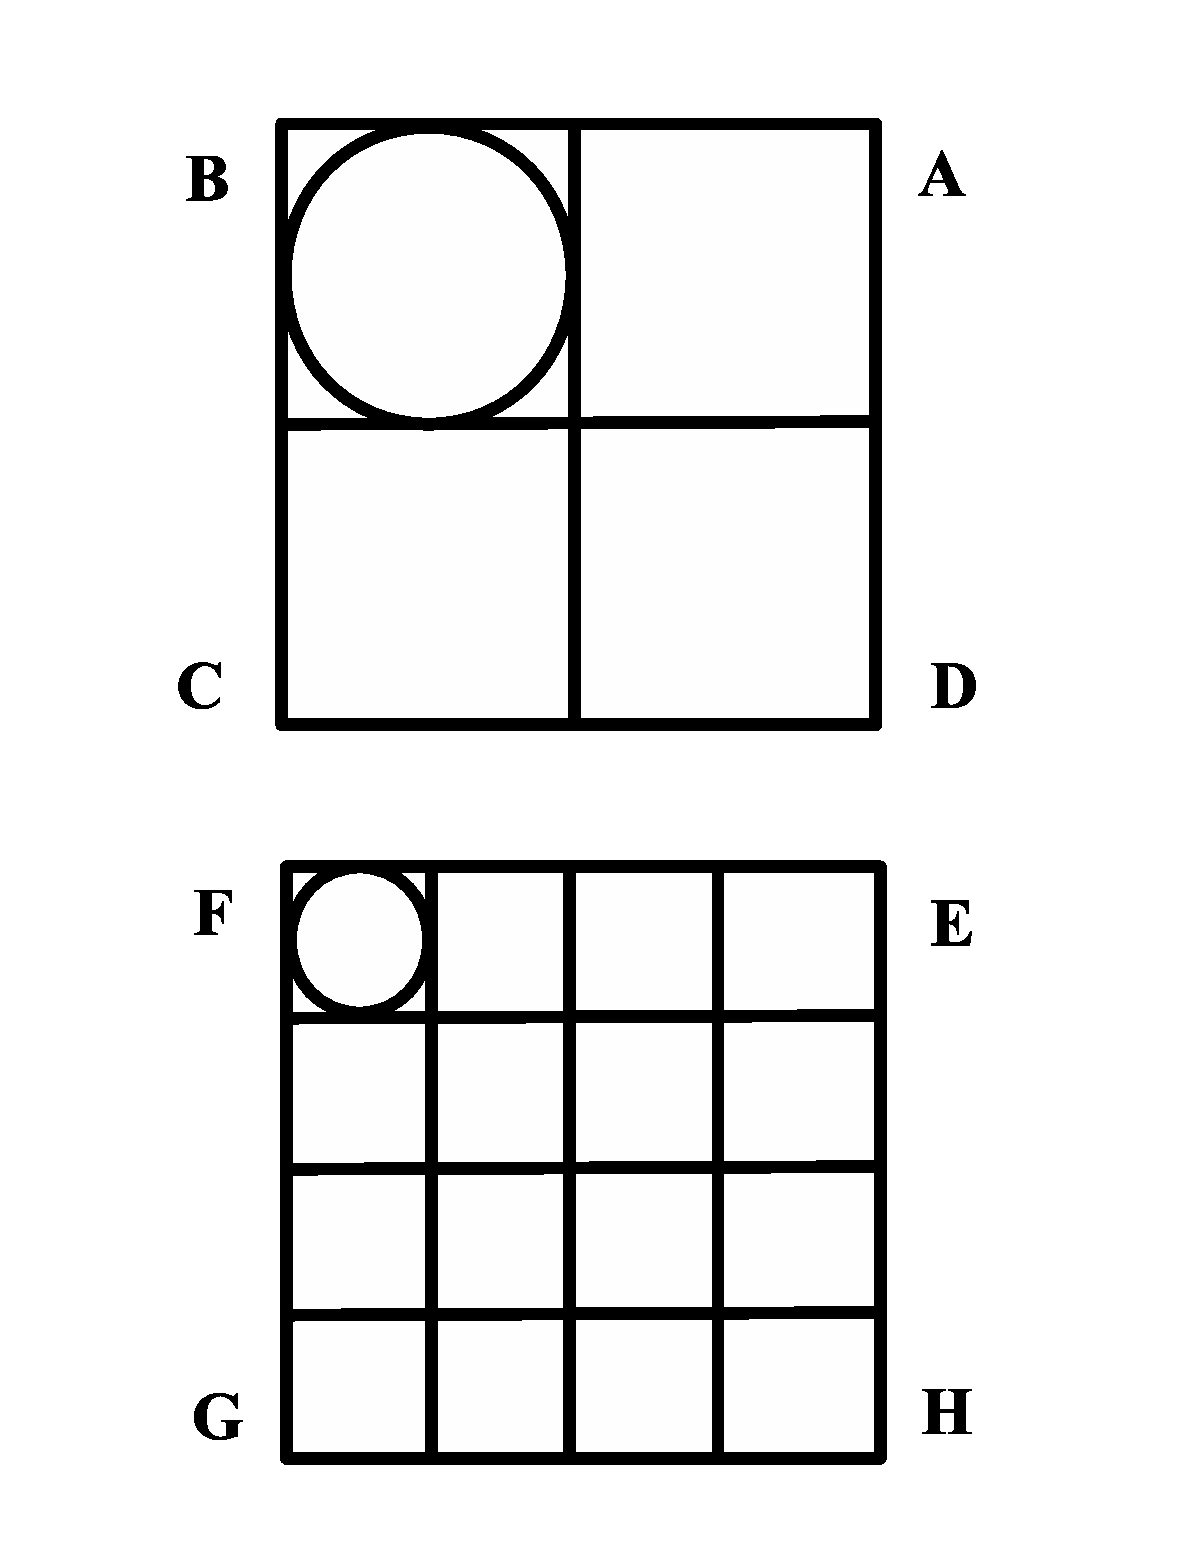
\includegraphics[width=20mm,viewport=66 28 464 700]{CCJPR74-20pic.eps}
\end{wrapfigure}

\textbf{The correct answer is (A): 4:1}\\[1 ex]
Let $D$ be the diameter of the large circle. The diameter of the small circle will then be $\frac{D}{2}$. Since the area of each large circle is
\begin{equation*}
\pi(\frac{D}{2})^2=\frac{\pi D^{2}}{4},
\end{equation*}
and the area of the small circle is
\begin{equation*}
\pi(\frac{\frac{D}{2}}{2})^2=\frac{\pi D^{2}}{16},
\end{equation*}
the ratio of the area of the large circle to the area of the small circle is 4:1.%End
\end{document}